\documentclass[11pt,a4paper]{article}

% Basic packages
\usepackage[fontset=fandol]{ctex}
\usepackage{amsmath, amssymb}
\usepackage{graphicx}
\usepackage[margin=2.15cm]{geometry}
\usepackage[most]{tcolorbox}
\usepackage{etoolbox}
\usepackage{listings}
\usepackage{hyperref}
\usepackage{booktabs}
\usepackage{subcaption}
\usepackage{float}
\usepackage{tikz}
\IfFileExists{pgfplots.sty}{
    \usepackage{pgfplots}
    \pgfplotsset{compat=1.18}
}{}

% Highlight box palette: low-saturation and print-friendly.
% Visual weight is ordered by teaching role, so a page mixing several boxes still
% reads important > warning > knowledge > dialogue instead of competing for attention.
% Title text is white on every title bar; contrast stays within WCAG AA (4.5:1--6.0:1).
\definecolor{kbBack}{HTML}{F2F6FA}\definecolor{kbFrame}{HTML}{9DB4CC}\definecolor{kbTitle}{HTML}{52708F}
\definecolor{ibBack}{HTML}{FBF5E7}\definecolor{ibFrame}{HTML}{C9A961}\definecolor{ibTitle}{HTML}{7D5F1E}
\definecolor{wbBack}{HTML}{FCF2F0}\definecolor{wbFrame}{HTML}{D6A096}\definecolor{wbTitle}{HTML}{9E4F43}
\definecolor{dbBack}{HTML}{F4F7F3}\definecolor{dbFrame}{HTML}{AEC2AC}\definecolor{dbTitle}{HTML}{5F7F64}

\tcbset{softbox/.style={
    enhanced, boxrule=0.8pt, arc=2pt, left=3mm, right=3mm, top=2mm, bottom=2mm,
    coltitle=white, fonttitle=\bfseries, toptitle=0.6mm, bottomtitle=0.6mm
}}

% Highlight boxes
\newtcolorbox{knowledgebox}[1]{
    softbox, colback=kbBack, colframe=kbFrame, colbacktitle=kbTitle, title=#1
}

\newtcolorbox{importantbox}[1]{
    softbox, colback=ibBack, colframe=ibFrame, colbacktitle=ibTitle, title=#1
}

\newtcolorbox{warningbox}[1]{
    softbox, colback=wbBack, colframe=wbFrame, colbacktitle=wbTitle, title=#1
}

\newtcolorbox{dialoguebox}[1]{
    softbox, breakable, colback=dbBack, colframe=dbFrame, colbacktitle=dbTitle, title=#1
}

% Listings
\lstset{
    language=Python,
    basicstyle=\ttfamily\small,
    keywordstyle=\color{blue},
    stringstyle=\color{red!60!black},
    commentstyle=\color{green!60!black},
    breaklines=true,
    frame=single,
    numbers=left,
    numberstyle=\tiny\color{gray},
    captionpos=b,
    extendedchars=false
}

\usepackage{tabularx}
\newcolumntype{L}[1]{>{\raggedright\arraybackslash}p{#1}}
\hypersetup{colorlinks=true,linkcolor=kbTitle,urlcolor=kbTitle,pdftitle={CMU L4 记忆与技能：中文课程讲义},pdfauthor={Based on Daniel Fried; Chinese notes prepared with Codex}}
\renewcommand{\baselinestretch}{1.13}
\setlength{\parskip}{.4em}
\setlength{\emergencystretch}{2em}
\setcounter{tocdepth}{1}
\captionsetup{font=small,labelfont=bf}
\lstset{basicstyle=\ttfamily\footnotesize,columns=fullflexible,keepspaces=true,xleftmargin=6mm,framexleftmargin=4mm}
\begin{document}
\special{pdf:minorversion 7}
\hypersetup{pageanchor=false}
\begin{titlepage}
\centering
\vspace*{.9cm}
{\Large CMU 11-768 · AI Agents\par}
\vspace{.6cm}
{\Huge\bfseries 记忆与技能\par}
\vspace{.4cm}
{\Large 从跨任务经验到可复用的行动知识\par}
\vspace{.5cm}
{\large L4 中文课程讲义\par}
\vspace{1cm}
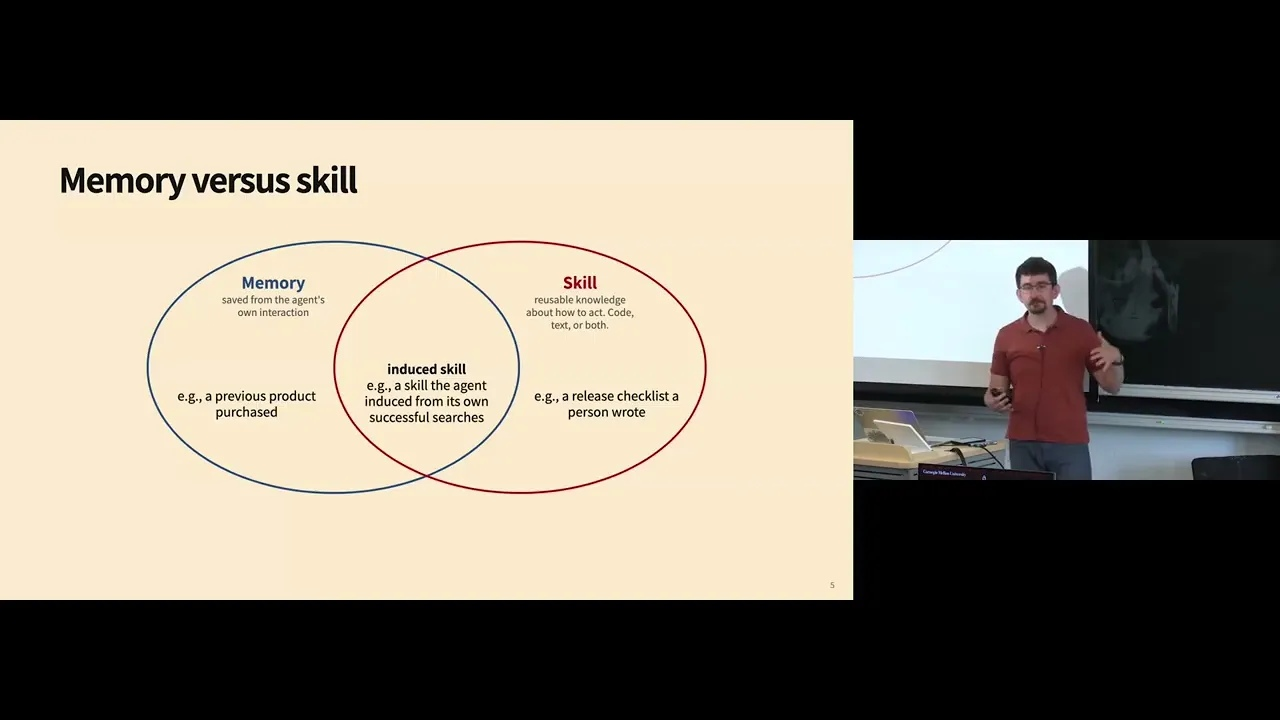
\includegraphics[width=\textwidth]{figures/原视频封面.jpg}\par
{\small 图：原视频封面\par}
\vfill
\begin{tcolorbox}[colback=kbBack,colframe=kbFrame,width=\textwidth]
\textbf{主讲}：Daniel Fried\par
\textbf{频道}：Graham Neubig\par
\textbf{课程}：Carnegie Mellon University，11-768 AI Agents，Fall 2026\par
\textbf{发布日期}：2026 年 9 月 8 日\par
\textbf{时长}：75 分 22 秒\par
\textbf{整理日期}：2026 年 10 月 4 日\par
\textbf{原视频}：\href{https://www.youtube.com/watch?v=6zigF2a-2Pw}{youtube.com/watch?v=6zigF2a-2Pw}
\end{tcolorbox}
\end{titlepage}
\pagenumbering{arabic}
\hypersetup{pageanchor=true}
\section*{本讲概览}
一次任务结束后，Agent 能留下什么，使下一次任务更容易完成？本讲从购物网站中反复出现的搜索步骤出发，讨论如何把交互经验保存为完整轨迹、事实、策略或可执行技能，以及这些表示如何进入后续任务。人工编写的技能提供已有知识；从经验归纳的技能则需要判断结果、提取共性、验证并持续维护。

讲义以原语言带时间字幕和 46 页官方课件为基础，结合原始论文与项目资料核对机制和实验条件。正文图示采用官方课件 PDF 裁图，保留原有矢量内容与嵌入图像，图注记录官方 PDF 页码及相关口述区间。代码说明用途与来源，实验数值保留任务、指标和评测设置；课堂略过或未展开的课件内容另作标注。

材料入口：\href{https://www.cmu-agents.com/slides/lecture-04-memory-and-skills.pdf}{官方课件}；\href{https://www.youtube.com/watch?v=6zigF2a-2Pw}{原视频}；\href{https://www.usetranscribe.io/yt/6zigF2a-2Pw/ai-agents-memory-skills}{公开带时间转录}。主要依据 YouTube 英文原语言自动字幕，结合课件纠正术语；各章提供相关原始资料链接。
\tableofcontents
\clearpage
% L4 body, part 1: 00:00--00:44:10, official slides 1--20.
% Figures are crops of the official PDF, not video screenshots.
\clearpage
\section{从重复任务出发：哪些经验值得留下？}
\label{sec:l4-experience}

\subsection{动机：完成一次搜索，下一次还要从头摸索吗？}

上一讲讨论的是同一任务内的上下文管理：智能体已经观察了什么、调用了什么工具、收到什么反馈，哪些内容应当继续留在模型的上下文窗口里。本讲把时间跨度拉长，问一个更接近日常工作的问题：\textbf{一次任务中获得的经验，怎样帮助下一次任务？}（00:00:36--00:02:00）

考虑同一购物网站上的两个请求。第一个请求是把 Sony 耳机加入愿望清单；第二个请求是报告无线键盘的价格范围。两个任务的结果不同，但都需要进入商店、找到搜索框、输入查询词、提交搜索。若第一次任务已经花了很多步骤才弄懂搜索入口，第二次再次探索这段流程就有重复成本。图\ref{fig:l4-shared-search}将共同过程与任务特有的收尾分开：查询词可以改变，共同的搜索结构仍可复用。

\begin{figure}[H]
\centering
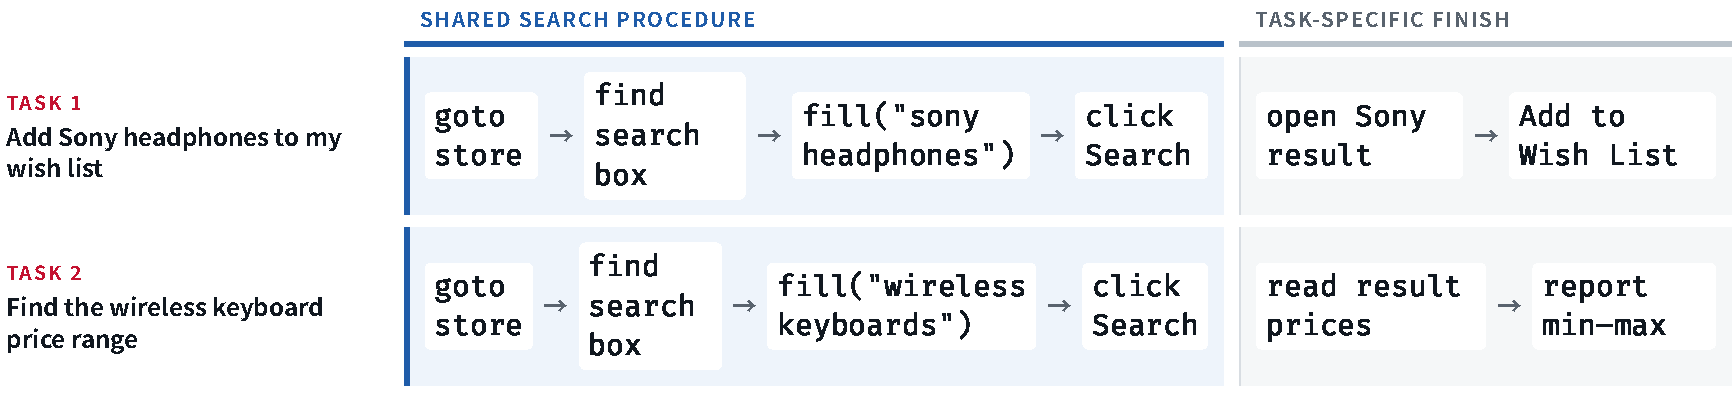
\includegraphics[width=0.99\textwidth]{figures/l4_shared_search_procedure.pdf}
\caption{两个购物任务共享搜索过程，随后分别加入愿望清单或读取价格。官方课件第2页裁图；相关口述：00:02:00--00:03:57。}
\label{fig:l4-shared-search}
\end{figure}

由此产生三个贯穿全讲的问题。\textbf{表示}：保存当时的动作序列、改写成自然语言步骤，还是抽象为可执行函数？\textbf{归纳}：怎样从一次成功操作中识别值得复用的部分，去掉产品名称等偶然细节？\textbf{生命周期}：何时检索、检查、修正或删除这段知识？把内容写进文件只是生命周期的起点。（00:03:13--00:04:40）

\begin{importantbox}{复用的对象是重复结构}
技能的价值来自未来任务会重复某个子过程。一次任务的所有细节都能被保存，但只有一部分细节值得成为以后执行任务的指导。搜索流程的复用并不意味着“加愿望清单”与“报告价格”也能互换。
\end{importantbox}

\subsection{机制：更新上下文、外部工件，还是模型权重？}

智能体的行为可以通过三个位置发生变化。它们对应不同的更新成本，也把不同责任交给了系统设计者。（00:04:40--00:07:21）

\begin{center}
\small
\begin{tabularx}{\textwidth}{p{2.4cm}XX}
\toprule
更新位置 & 主要收益 & 主要负担 \\
\midrule
上下文窗口 & 直接保留观察、动作、用户消息与反馈，细节忠实 & 长轨迹占用大量 token；噪声与相关内容混杂；需要选择和压缩 \\
外部工件 & 文件或数据库可被检查、编辑、检索，并可交给其他模型使用 & 必须决定保存什么、什么时候取回，以及如何维护冲突和过时内容 \\
模型权重 & 通过监督微调或强化学习形成较广泛的行为变化，减少反复提供同类指导的需要 & 更新更慢；内部变化较难检查；更新依附于特定模型 \\
\bottomrule
\end{tabularx}
\end{center}

外部工件提供了一个清楚的人机协作接口。人可以查看智能体总结出的“如何在这个网站搜索”，修改其中的错误，再交给另一个模型使用。相对地，对一个模型做了权重更新，另一个模型不会自动获得同样的变化。这里的“可迁移”指工件可以被传递和解释，\textbf{不保证每个模型都会同样正确地理解或执行它}。

即使上下文窗口很长，跨很多任务积累的历史仍可能超过窗口，更关键的是，历史越多，模型越需要分辨哪些内容与当前任务相关。外部存储解决容量和持久化问题，检索与维护才决定其中的内容能否真正改善行为。

\subsection{例子：episode、fact 与 skill 保留了不同粒度}

同一次购物操作可以留下三类经验。（00:09:00--00:11:35）

\begin{itemize}
\item \textbf{完整经历（episode）}：保留用户要求、页面观察、每次动作、工具结果与最终结局。它适合以后需要核对某个具体商品、某个当时价格或当时操作顺序的情况，代价是保存和读取都较昂贵。
\item \textbf{事实（fact）}：例如“这个商店只有进入商品详情页才显示价格”。它压缩了经历中的一条环境知识，可帮助多种任务，也可能随网站变化而失效。
\item \textbf{技能（skill）}：例如“填写搜索框、提交搜索、打开符合条件的结果”。它保留如何行动的过程，并把产品名称之类的变量留给新任务。
\end{itemize}

同一条事实可以被多个技能利用；同一段技能也可以从多条经历中归纳出来。因此，这三个词表达的是不同的保存粒度与用途，实际系统可以同时拥有它们。

图\ref{fig:l4-memory-skill}进一步区分来源与用途。\textbf{记忆}强调从智能体自己的交互中保存的内容；\textbf{技能}强调可重复使用的行动知识。人写的发布检查清单是技能，购买过哪件商品是记忆，从成功搜索中归纳的搜索方法则位于二者交集。

\begin{figure}[H]
\centering
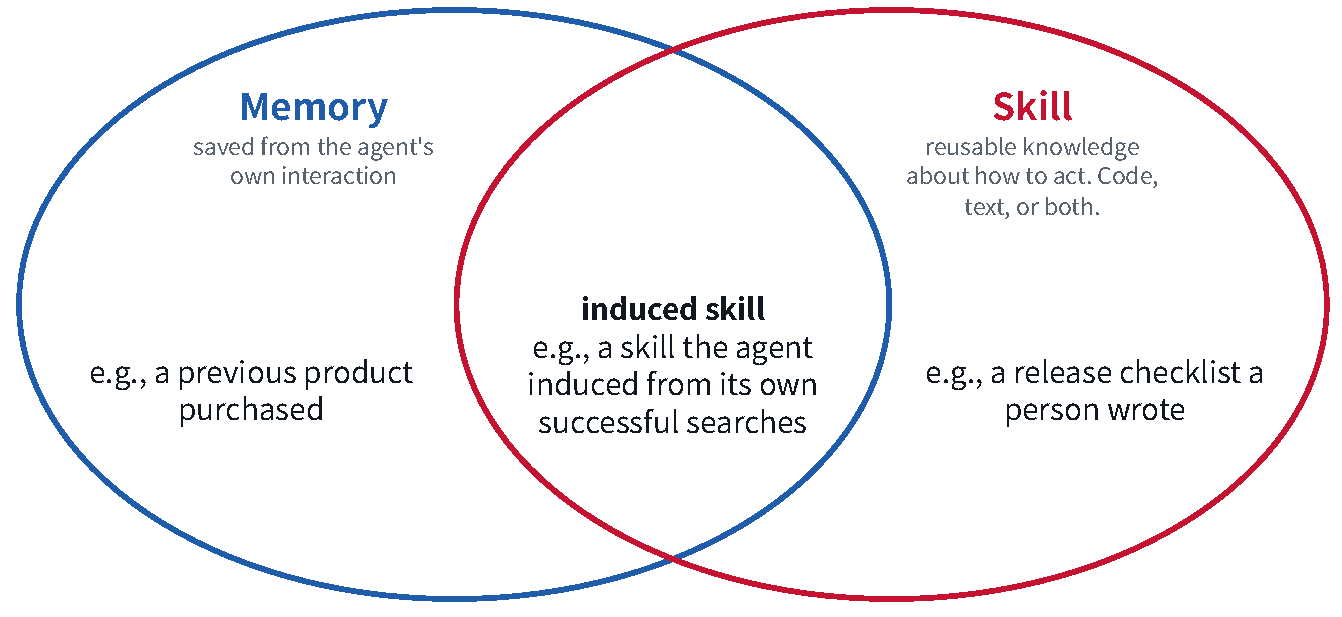
\includegraphics[width=0.90\textwidth]{figures/l4_memory_skill_overlap.pdf}
\caption{记忆与技能可以相交：智能体从自身经历中归纳出的行动方法是 induced skill。官方课件第5页裁图；相关口述：00:11:35--00:12:54。}
\label{fig:l4-memory-skill}
\end{figure}

\subsection{证据与边界：人工编写和从经历学习可以互相补充}

课程先讨论人工编写技能，再讨论智能体从经历归纳技能。前者把专业知识、组织约定和工作偏好显式交给智能体，来源与意图比较清楚，但编写和维护需要人的时间。后者从实际 episode 与结果出发，适合操作方法必须在环境中探索的场景，但需要判断结果、验证归纳内容，并筛选入库。（00:12:54--00:14:15）

这两条路径可以组合：智能体先提议一条操作经验，人编辑后采用；人先写出一条规范，智能体再根据实际执行中的反馈提出修改。学习因而可以发生在外部工件上，模型权重保持不变也能改善下一次行为。

\begin{warningbox}{课堂经验：技能写得过多会扩大任务}
在00:07:36--00:09:00的课堂交流中，有同学报告：模型生成技能时会推断出过多要求，交给另一个模型后，后者逐条照做，执行了超出原意的工作。另一位同学提到，可把过去几次支持处理的过程交给模型，让它整理成供其他智能体使用的说明。讲者据此强调：明确让模型考虑“另一个执行者将如何理解这些说明”，有助于改善指令表达；生成后仍需检查适用范围。
\end{warningbox}

\subsection{本章小结}

本讲关注跨任务的行为改善。首先应识别未来还会出现的共同结构，然后选择保存完整经历、事实还是行动技能。外部工件易于检查、编辑和传递，但这些优点同时带来保存、检索、验证与维护的责任。人工技能与归纳技能的来源不同，可以通过共同的外部表示形成协作循环。

\clearpage
\section{人工编写技能：把固定规范变成可按需读取的资源}
\label{sec:l4-authored}

\subsection{动机：反复输入的审查要求可以形成技能}

课程用 Python 代码审查作为人工技能的例子：每次审查都要求 Black 的88字符行宽、采用团队的 Ruff 规则、公共 API 带类型标注、使用 Google 风格 docstring，并为新函数使用 Pytest。反复重新输入同一套要求容易遗漏，也不方便修改。把要求保存为一个技能包，智能体以后遇到相同类别的工作时就可以读取这套规范。（00:14:15--00:15:31）

\begin{importantbox}{人工技能的基本用途}
当一类工作要反复遵循固定规范时，可以把流程、约定与必要资源封装为技能。技能既能提供文字指导，也能带来自动化脚本；模型仍需根据当前任务解释哪些步骤适用。
\end{importantbox}

此处的88字符、工具选择和“所有新函数”是\textbf{课件展示的团队规范}，读者不应把它们当成所有项目的通用审查政策。技能的职责是把某个明确环境中的规范传递给执行者。

\subsection{机制之一：一个技能包怎样组织文件？}

课件采用 Agent Skills 风格的文件包。必要入口是\texttt{SKILL.md}，文件开头是 YAML 元数据，随后是 Markdown 正文；脚本、参考资料与静态资源可以作为附带文件。（00:15:31--00:17:32）下面的目录是根据课件整理的教学例子。

\par\noindent\begin{minipage}{\linewidth}
\begin{lstlisting}[language={},caption={教学例子：Python审查技能的文件组织}]
python-review/
  SKILL.md
  scripts/
    run_checks.py
  references/
    docstring-style.md
  assets/
    review-template.md
\end{lstlisting}
\end{minipage}

\texttt{scripts/}放可执行代码，例如检查格式与静态规则的脚本；\texttt{references/}放不必每次全部读取的详细规则；\texttt{assets/}放模板等资源。目录约定帮助组织内容，真正使资源可被找到的是\texttt{SKILL.md}中的说明与引用。

下面只示范核心元数据与正文的连接。正文告诉模型做什么，并指出执行工具和详细文档在哪里。示例经过教学改写，不是产品的完整技能模板。

\par\noindent\begin{minipage}{\linewidth}
\begin{lstlisting}[language={},caption={教学例子：元数据帮助选择，正文指导执行}]
---
name: python-review
description: Review Python changes against repository conventions.
  Use for Python code review and style checks.
---
# Python review
Read the repository conventions before reviewing changes.
Run scripts/run_checks.py on the changed Python files.
Check public API type hints and docstrings.
See references/docstring-style.md when detailed rules are needed.
Use assets/review-template.md to organize the final review.
\end{lstlisting}
\end{minipage}

\begin{warningbox}{课件中的\texttt{triggers}不等于跨框架标准}
第9页示例含有\texttt{triggers}列表。核对\href{https://agentskills.io/specification}{Agent Skills原始规范}后，必需元数据是\texttt{name}与\texttt{description}；规范未把\texttt{triggers}列为标准字段。应把适用时机写进描述，具体框架是否识别额外字段、怎样触发加载，需要查看该框架实现。字段名称本身不会让技能自动执行。
\end{warningbox}

\subsection{机制之二：渐进加载控制上下文成本}

如果把所有技能正文、脚本和参考文档同时放进上下文，技能库越大，任务的工作空间就越小。渐进加载（progressive disclosure）把“知道资源存在”与“读入资源细节”分开。（00:17:32--00:19:05）

\begin{enumerate}
\item \textbf{先显示索引。}模型先看到可用技能的名称和简短描述，在课程展示的实现中，这些内容进入系统提示词。
\item \textbf{相关时读取正文。}模型判断当前请求需要某个技能，调用工具读取\texttt{SKILL.md}，工具结果把具体步骤带进上下文。
\item \textbf{按需使用附带资源。}正文提示还有哪些脚本与文档；执行者遇到具体需要时，再读取参考文件或运行脚本。
\end{enumerate}

图\ref{fig:l4-progressive-loading}展示四个不同的上下文增量。加载技能正文得到审查步骤；运行检查脚本得到 Black 与 Ruff 的检查结果；读取 docstring 参考文件才得到详细文档规则。\textbf{执行脚本不要求先把脚本源代码全部放进模型上下文}，工具可以在外部执行代码，再把输出交回模型。若模型主动查看脚本源文件，源代码当然也会进入上下文。

\begin{figure}[H]
\centering
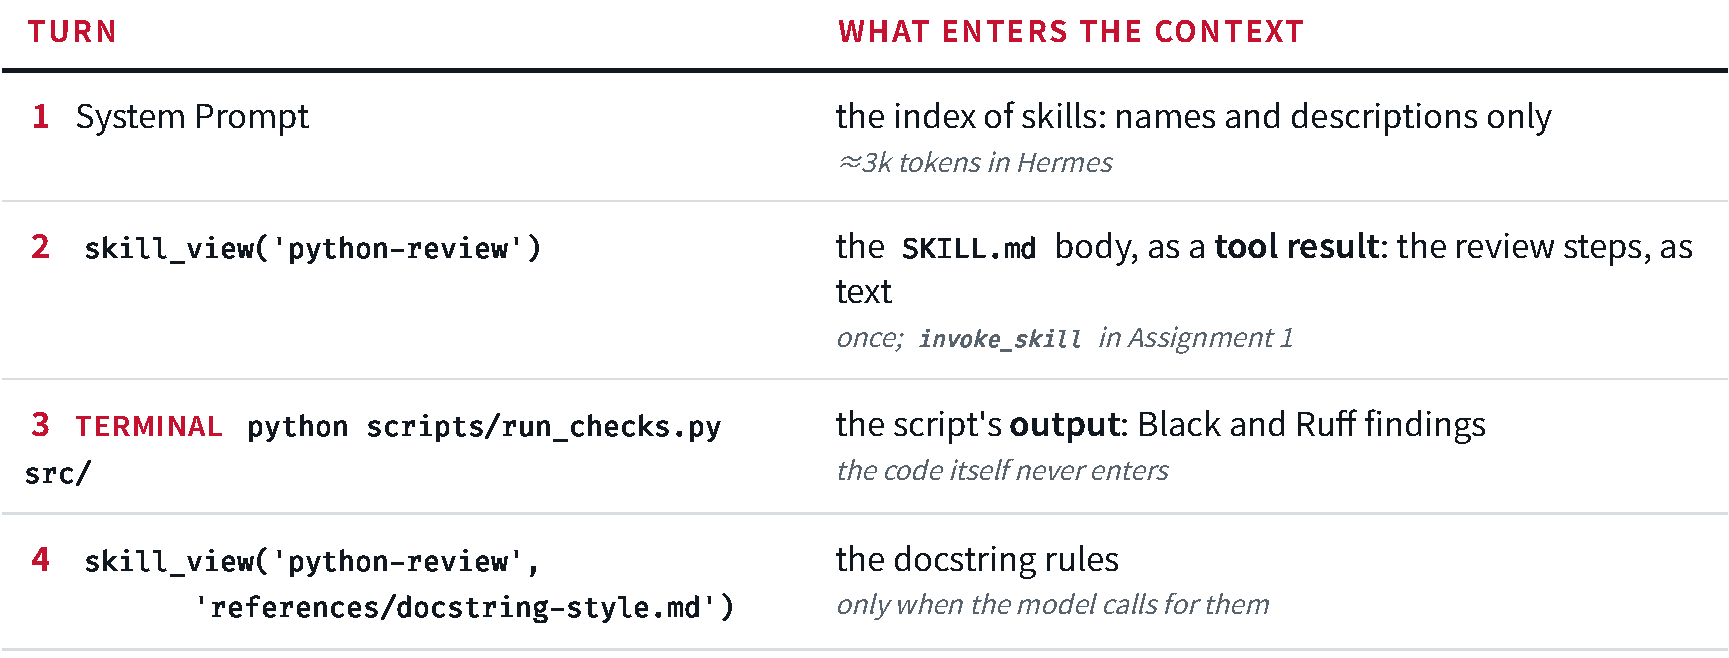
\includegraphics[width=0.99\textwidth]{figures/l4_progressive_loading_context.pdf}
\caption{课程中的Hermes示例区分了索引、正文、脚本输出与按需参考文档。官方课件第11页裁图；相关口述：00:24:26--00:26:13。}
\label{fig:l4-progressive-loading}
\end{figure}

课程第10页还展示了 Hermes 的索引提示词：向模型说明技能机制、提供\texttt{skill\_view}工具，再列出可用技能。第11页指出课程作业中类似接口名为\texttt{invoke\_skill}。\textbf{这些是课堂实例的工具名称，接口命名与是否重复加载由实现决定。}同样，图中索引约3千 token 是讲者对该实例的描述，不是所有技能系统的固定开销。

\begin{importantbox}{渐进加载解决“何时把什么内容放进上下文”}
索引负责可发现性，正文负责行动指导，附带资源负责细节与执行。入口正文需要足够短，也需要清楚地指向关键资源；否则虽然资源已打包，模型仍可能不知道应当读取它。
\end{importantbox}

\subsection{课堂问答：触发、格式和大规模技能库}

\textbf{技能很多，只有元数据也会影响性能吗？}（00:19:05--00:20:19）会。索引也占用上下文，模型还可能被无关描述吸引。渐进加载减少正文的成本，却没有消除索引规模问题。讲者提出让技能数量保持可管理，或根据任务条件先选择一部分技能。

\textbf{触发对描述有多敏感？}（00:20:19--00:20:59）是否产生读取技能的工具调用依赖模型、当前上下文及描述的写法。描述有关键词并不等于字符串匹配成功就会可靠触发；需要评估模型是否在正确场景加载、并在加载后正确使用。

\textbf{必须用\texttt{SKILL.md}和Markdown吗？}（00:20:59--00:23:10）标准文件名方便框架发现入口；Markdown同时照顾人阅读和模型解释，可包含链接、示例与图像。动态过程或交互式可视化可以由代码资源承载，并在正文中引用。课堂进一步指出，文字技能可放正文，程序技能可放脚本，文件包能容纳二者。

\textbf{数目极大的基础设施工具或技能怎样处理？}（00:23:10--00:25:14）讲者给出两种研究中常见的选择方式：用文本向量检索与当前任务接近的技能，或按域选择，例如当前在哪个网站就只加载该网站相关的技能。这里给出的是设计方向；讲者没有提供一个适用于所有生产系统的统一检索实现。

\subsection{本章小结}

人工技能把反复出现的规范保存为可复用资源。文件包提供统一入口，并把正文、脚本和资料分层组织；渐进加载让模型先看到可选项，再逐步获取所需细节。描述、加载工具与框架行为共同决定技能是否被采用，因此“文件存在”“被加载”“被正确执行”应分别检查。

\subsection{拓展阅读}

\begin{itemize}
\item \href{https://agentskills.io/specification}{Agent Skills specification}：用于核对入口文件、元数据和渐进加载约定；本文对标准字段的校核依据。
\item \href{https://www.anthropic.com/engineering/equipping-agents-for-the-real-world-with-agent-skills}{Equipping agents for the real world with Agent Skills}：课件采用的渐进加载说明来源。
\end{itemize}

\clearpage
\section{技能是否有效：用评估和反馈维护技能}
\label{sec:l4-evaluation}

\subsection{动机：读到了技能，为什么结果仍可能变差？}

前一章解决了技能如何被组织和送入上下文，接下来要验证它带来的行为变化。技能可能提供模型原本不知道的专业流程，也可能让模型放弃更合适的默认做法；它可能缩短执行，也可能增加无关步骤。因此，评估问题应具体到\textbf{某项任务、某套技能内容，以及某个模型和执行框架的组合}。（00:26:13--00:29:12）

\subsection{机制与证据：SkillsBench怎样比较“有技能”和“无技能”？}

课程采用的 SkillsBench 版本包含87个真实工作任务、8个领域和18种模型与框架配置。研究先收集大规模技能库，并独立收集候选任务，再经过质量检查和人工审阅，形成\textbf{任务与技能包的人工配对}。主实验对同一任务比较无技能与提供精选技能包的条件，使用编写好的验证程序判断结果。（官方课件第12--13页）

\begin{figure}[H]
\centering
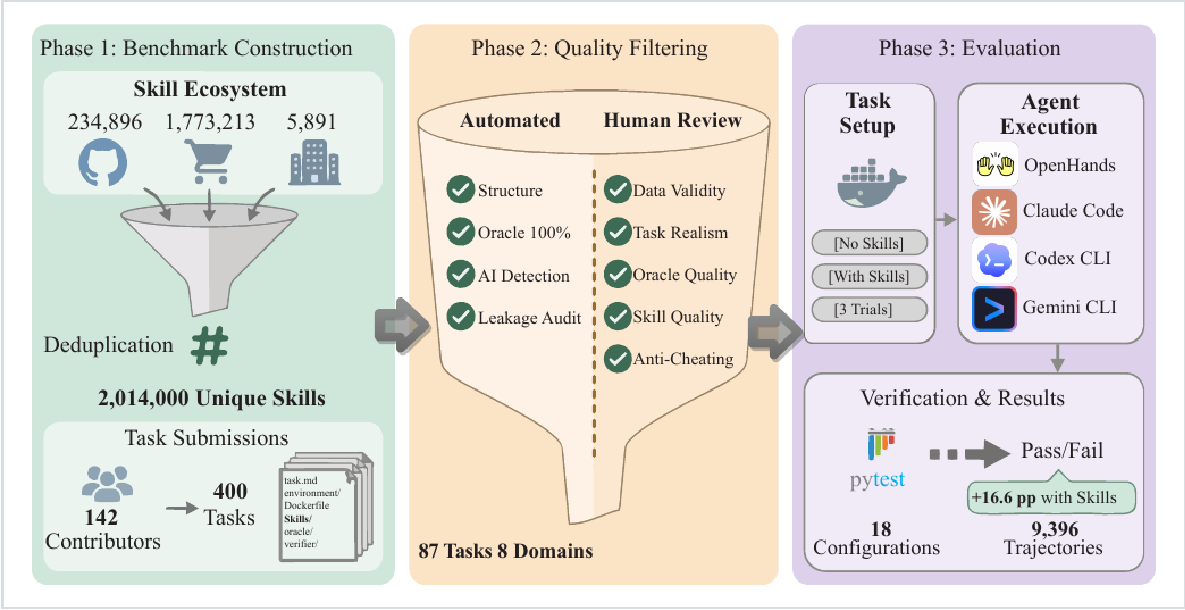
\includegraphics[width=0.94\textwidth]{figures/l4_skillsbench_construction_evaluation.pdf}
\caption{SkillsBench从候选技能与任务经过过滤，得到87个任务，并对模型与框架组合进行匹配条件的评估。官方课件第12页裁图；相关口述：00:26:13--00:28:15。}
\label{fig:l4-skillsbench-pipeline}
\end{figure}

图\ref{fig:l4-skillsbench-pipeline}中的过滤步骤包括结构检查、参考解能否通过验证、技能是否泄漏特定任务答案，以及技能与任务是否真实、合理。这样做的目的，是让技能提供可复用的过程知识，同时让验证器评价实际输出。

\begin{warningbox}{精选技能包的效果不等于全库自动发现的效果}
人工已经挑选了供应给每个任务的技能包。智能体仍须发现并使用包内内容，但主实验没有证明它能从数百万个候选技能中自动挑出正确的一组。任务进入评测还经过质量与信号筛选，结果应解释为该基准中的技能收益，不能直接外推为任意来源技能的平均收益。
\end{warningbox}

图\ref{fig:l4-skillsbench-results}显示不同组合的基线与技能后结果。平均通过率从33.9\%上升到50.5\%。为了避免把百分比和百分点混为一谈，可以直接写出差值：

$$
\Delta = p_{\mathrm{skill}}-p_{\mathrm{base}}
       = 50.5\%-33.9\% = 16.6\text{ 个百分点}.
$$
\begin{itemize}
\item $\Delta$：加入精选技能后的通过率绝对增量，以百分点表示。
\item $p_{\mathrm{skill}}$：提供精选技能包条件下的平均通过率，这里为50.5\%。
\item $p_{\mathrm{base}}$：无技能条件下的平均通过率，这里为33.9\%。
\end{itemize}

\begin{figure}[H]
\centering
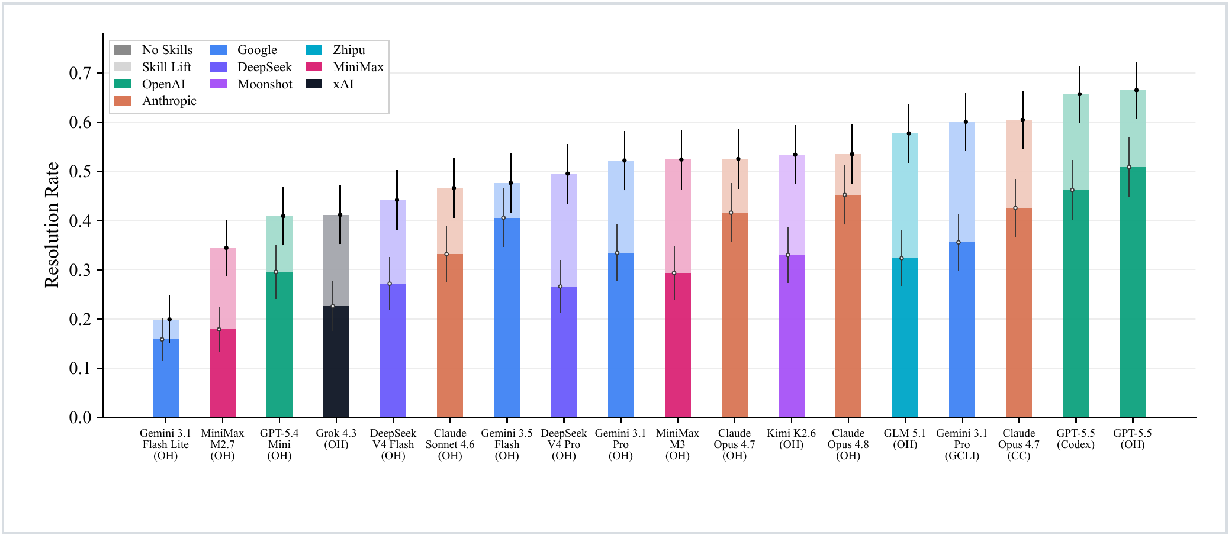
\includegraphics[width=\textwidth]{figures/l4_skillsbench_configuration_results.pdf}
\caption{不同模型与框架组合的通过率。图例区分无技能基线及加入技能后的提升，收益大小随组合变化。官方课件第13页裁图；相关口述：00:28:15--00:29:12。}
\label{fig:l4-skillsbench-results}
\end{figure}

\textbf{数字版本说明。}本节采用课件给出的87任务、8领域、18配置和16.6百分点。制作时核对的\href{https://arxiv.org/html/2602.12670}{SkillsBench原始论文HTML}与这些数字一致（访问日期：2026年10月4日）；早期论文版本的任务规模和汇总数字不同，跨版本比较前应先对齐评测集合与配置。

\subsection{边界：少量聚焦技能的收益是观察结果}

课件指出，配置1--3个技能的任务通常比配置至少4个技能的任务获得更大提升，较短的\texttt{SKILL.md}组也显示较大收益。这提示聚焦内容更容易被模型利用。然而，不同组可能对应不同任务难度与组成，\textbf{该分组关系不能单独证明“删到3个技能就一定更好”}。讲者提出的解释包括更多技能带来的干扰，也包括任务本身更难。（00:28:15--00:29:12）

87个任务中仍有13个在加入技能后出现负向差值。一个流程即使看似正确，也可能不适合当前请求，或让模型采用比默认做法更笨重的策略。为新场景采用技能时，检查任务成功与失败，并观察是否执行了额外步骤，比只确认技能文件已加载更有意义。

课程还提到“让模型仅凭任务描述先写技能，再完成任务”的实验条件，其效果可能更差。这个结果针对的是这种\textbf{先验生成条件}，并不等于从真实交互与反馈归纳技能没有价值。后者正是后续课程要展开的主题。（00:30:06--00:30:47）

\subsection{实例：OpenHands如何维护代码审查技能？}

技能可以随框架附带，可以由人编写、从其他仓库安装，也可以由智能体根据刚完成的流程起草。课件举到 Hermes 的\texttt{skill\_manage}与 OpenHands 的\texttt{/skill-creator}；这些是课程使用的实现实例。课程建议在重复流程完成后趁上下文完整时整理技能，再试用几次，让实际执行暴露遗漏与歧义。（00:29:12--00:30:47）

接下来，OpenHands 的代码审查案例展示了持续维护的做法：每次运行留下日志；PR 合并后，结合人类反馈与最终代码判断哪些建议被采用；汇总很多运行中的失败模式；让模型提议修改\texttt{SKILL.md}。（00:30:47--00:32:40）

\begin{figure}[H]
\centering

\includegraphics[width=\textwidth]{figures/l4_review_skill_maintenance_loop.pdf}
\caption{代码审查技能从使用、记录、评分到修补的维护闭环。官方课件第15页裁图；相关口述：00:30:47--00:32:40。}
\label{fig:l4-review-loop}
\end{figure}

这个案例使用的一个信号是建议采纳比例：模型判定审查中有多少可执行建议，再检查其中多少体现于人的回复或合并后的修改。直观上，建议经常被实际采用，说明它更贴近团队需求。

$$
A = \frac{N_{\mathrm{kept}}}{N_{\mathrm{suggested}}}.
$$
\begin{itemize}
\item $A$：建议采纳比例，用于监测代码审查输出的实用性。
\item $N_{\mathrm{kept}}$：被人类反馈或最终修改认定为已采纳的可执行建议数量。
\item $N_{\mathrm{suggested}}$：智能体提出的可执行建议总数；当其为0时，该次运行不能直接用上述比值评分。
\end{itemize}

课件与原案例列出两种反复出现的问题。第一种是忽略仓库约定，例如提出技术上合理、却不符合该仓库测试或依赖维护方式的建议；原文示例分析估计它占\textbf{有建议的轨迹约15\%}。第二种是在发现严重缺陷后仍批准 PR；示例分析估计约占\textbf{轨迹的10\%}。两者统计口径不同，也都是案例中的近似频率，不能当作所有代码审查智能体的普遍错误率。

对应修补很具体：发现关键问题时应要求修改；发布建议前先检查仓库已有模式和事实。维护由此落到一条可以改变下一次行为的指令上，而不只是一份“本次做得不好”的分析。

\begin{knowledgebox}{采纳比例有价值，也有盲区}
采纳信号衡量建议是否被实际使用，无法独立衡量遗漏了多少严重问题。人未采纳也可能有其他原因；模型判官对“是否采纳”的判断也可能有误。课程案例的启发是把指标与运行日志、失败分析结合，用它定位具体修补点。这里的指标解释是教学补充，课堂没有给出其全部统计局限。
\end{knowledgebox}

\subsection{本章小结}

技能效果需要通过匹配条件比较，且与模型、框架和任务共同相关。SkillsBench说明精选技能在该评测中平均有效，同时保留了会变差的任务和分组差异。实际维护应把输出、反馈、评分、失败模式与技能更新连接起来；每次修补都应有一个能观察到的行为目标。

\subsection{拓展阅读}

\begin{itemize}
\item \href{https://arxiv.org/html/2602.12670}{SkillsBench: Benchmarking How Well Agent Skills Work Across Diverse Tasks}：本节统计口径与版本校核来源。
\item \href{https://www.openhands.dev/blog/20260227-creating-effective-agent-skills}{How to Create Effective Agent Skills}（Michelini与Neubig，2026）：代码审查维护案例与建议采纳指标的原始说明。
\end{itemize}

\clearpage
\section{自动记忆的基础：事实管理、反思与相似轨迹}
\label{sec:l4-memory-foundations}

\subsection{动机：外部存储只有被正确读写，才会影响行动}

人工技能提供了可复用知识，但跨任务学习还需要智能体自己保存经历。在归纳更抽象的技能之前，课程先介绍三种基础能力：\textbf{把信息在上下文和外部存储之间移动，保持事实一致，以及利用已有轨迹和反馈指导下一次尝试}。（00:32:40--00:33:48）

这三个问题的时间跨度不同。事实可能跨多次对话更新；反思通常先帮助同一任务的下一次重试；轨迹检索则为一个新任务提供过去相似任务的示例。理解差别，才能知道一份“记忆”究竟保存了什么、怎样起作用。

\subsection{MemGPT：模型通过函数调用管理记忆层级}

MemGPT（Packer等，2023）借用了操作系统的分层存储思路：上下文窗口里的内容可以直接被模型使用，容量较大的外部存储则需要先检索、再带回上下文。论文提出时窗口较短，图\ref{fig:l4-memgpt-hierarchy}以8千 token 为例；这是历史示意容量，机制并不依赖某个固定窗口大小。（00:32:40--00:35:06）

\begin{figure}[H]
\centering
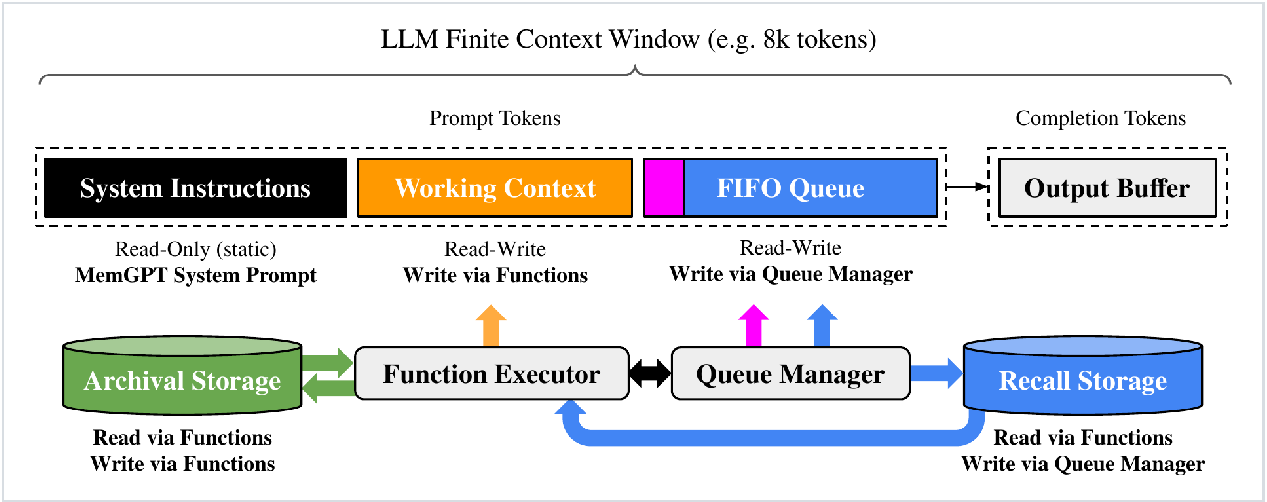
\includegraphics[width=\textwidth]{figures/l4_memgpt_memory_hierarchy.pdf}
\caption{MemGPT的系统指令、可读写工作上下文、FIFO消息队列与外部存储。官方课件第17页裁图，转引原论文图；相关口述：00:32:40--00:34:21。}
\label{fig:l4-memgpt-hierarchy}
\end{figure}

主上下文包括只读的系统指令、可通过函数修改的工作上下文，以及滚动保存近期消息的 FIFO 队列。外部层又有两类存储：\textbf{archival storage}保存可读写的长期文本内容；\textbf{recall storage}保留对话消息，便于查找以前发生过的交互。函数执行器与队列管理器负责把模型发出的调用落实为数据移动。

这里必须区分“模型选择读写”与“存储自己影响模型”：模型根据当前任务生成读写函数调用，执行器处理调用，检索结果成为新的上下文内容，随后模型才能据此回答。图\ref{fig:l4-memgpt-recall}给出具体例子：用户提到 Six Flags 时，系统搜索历史消息，找到以前关于该地点的交流，再把这些结果交给模型。

\begin{figure}[H]
\centering
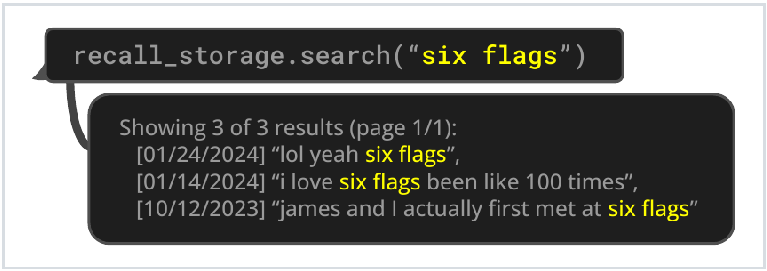
\includegraphics[width=0.86\textwidth]{figures/l4_memgpt_six_flags_recall.pdf}
\caption{以\texttt{six flags}为查询的历史消息检索；结果包含不同日期的相关交流。官方课件第17页裁图；相关口述：00:34:21--00:35:06。}
\label{fig:l4-memgpt-recall}
\end{figure}

\begin{importantbox}{外部记忆需要显式的数据通路}
信息存在数据库里，并不意味着语言模型当前已经知道它。读写工具、查询结果和工作上下文共同构成使用记忆的机制。课程在这里强调的是记忆管理控制权可以交给模型，而不是每个事实都必须由人在提示词中手动维护。
\end{importantbox}

\subsection{Mem0：先提取候选事实，再与已有记忆协调}

只会添加记忆，会让旧事实与新事实同时存在。例如用户先说在公司 X 工作，后来换了工作，模型需要使用更新后的状态；若用户说已经离职，继续把“目前在 X 工作”作为事实就会误导回答。Mem0（Chhikara等，2025）将记忆写入分成提取和更新两阶段。（00:35:06--00:37:01）

\begin{figure}[H]
\centering
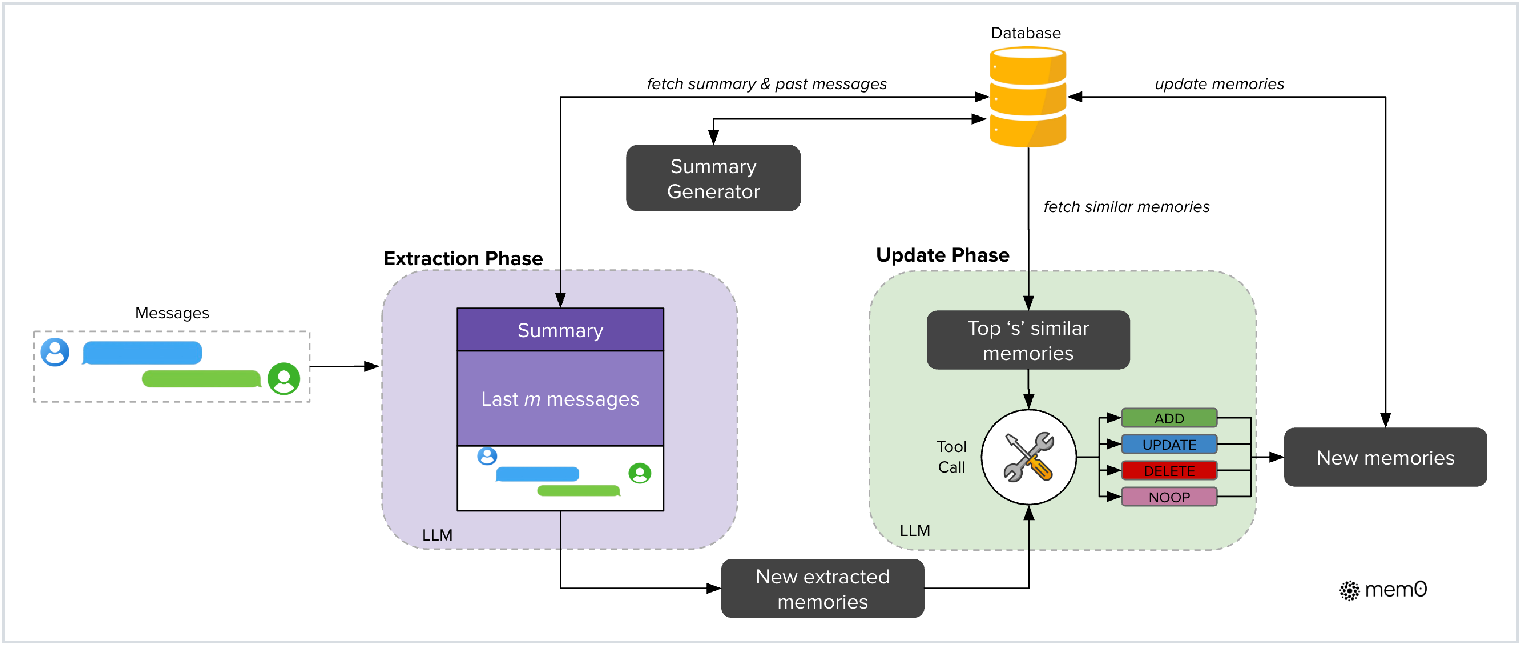
\includegraphics[width=\textwidth]{figures/l4_mem0_extract_reconcile.pdf}
\caption{Mem0先从消息及历史上下文提取候选事实，再检索相似记忆并选择更新操作。官方课件第18页裁图，转引原论文图；相关口述：00:35:06--00:37:01。}
\label{fig:l4-mem0}
\end{figure}

第一阶段从新消息中提取可能值得保存的内容，利用会话摘要和近期消息消除局部语境歧义。第二阶段对每条候选事实做向量检索，得到已有存储中最相近的一组记忆，再把新旧内容交给模型判断。相似检索先缩小比较范围；\textbf{是否冲突、重复或补充信息，仍是语义判断}，不能由向量相似度直接替代。

\begin{center}
\small
\begin{tabularx}{\textwidth}{p{1.65cm}Xp{4.8cm}}
\toprule
操作 & 语义目的 & 教学例子 \\
\midrule
\texttt{ADD} & 没有相应事实，加入新记忆 & 首次说“我住在上海” \\
\texttt{UPDATE} & 对已有记忆做补充或变更 & 为已知工作信息补充职位，或维护当前状态 \\
\texttt{DELETE} & 新信息否定已有记忆，移除过时内容 & 已离职，移除“目前在公司X工作” \\
\texttt{NOOP} & 已经保存、或无需修改记忆 & 重复确认同一条事实 \\
\bottomrule
\end{tabularx}
\end{center}

表中例子为教学说明。课程对\texttt{UPDATE}采用较宽的“变更已有事实”说法；原论文还强调补充更丰富的信息，并以\texttt{DELETE}处理被否定的记忆。具体系统对“换工作”可能采用删除旧当前状态后添加新状态，也可能更新同一记录，关键是避免新旧当前状态并存为矛盾事实。

\begin{warningbox}{当前事实与历史事实应区分}
“用户曾在X工作”与“用户现在在X工作”有不同含义。新消息否定当前状态，不自动否定这段历史。课程用离职说明删除的动机；在需要历史推理的系统里，还应考虑记录时间与有效状态。此处是由例子引出的教学边界，并非课堂规定的统一数据结构。
\end{warningbox}

\textbf{课堂连接：为什么需要遗忘或覆盖？}（00:37:01--00:38:32）讲者让同学回想上一讲可以修改记忆的机制，讨论到 Delta 类线性注意力对特定查询关联值的覆盖。本节在文本事实层处理冲突，上一讲在向量状态层处理覆盖，两者都有“记忆不能永远只追加”的动机。它们的数据结构和计算机制不同，类比不应解释为同一个算法。讲者随后也提到权重更新中可能需要遗忘冲突知识，unlearning 是相关研究方向。

\subsection{Reflexion：把失败信号变成同一任务的下一次指导}

事实管理关心“知道什么”，Reflexion（Shinn等，NeurIPS 2023）关心“这次为何失败，下一次怎样改”。一次尝试结束后，评价器给出结果信号；反思模块结合任务、轨迹与反馈生成自然语言建议；下一次尝试将该建议纳入上下文。（00:38:32--00:40:53）

评价器与反思模块承担不同职责。前者判断结果是否成功，可以来自环境、人的检查或模型判官；后者把笼统的“失败”解释为可行动的原因。反思文本的价值，来自它使下一次尝试知道该改变哪一处判断或操作。

\begin{figure}[H]
\centering
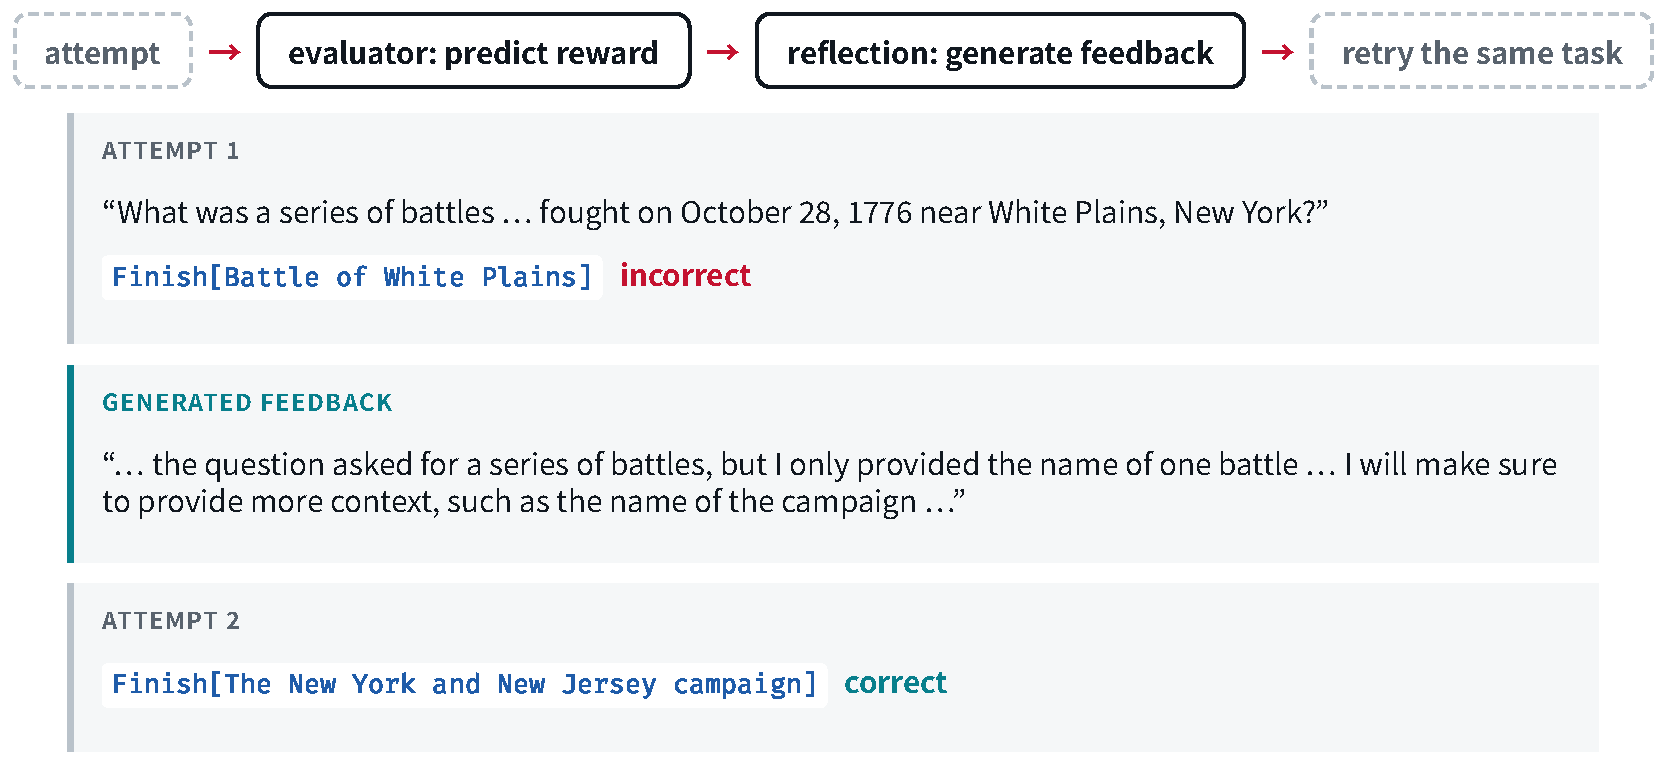
\includegraphics[width=\textwidth]{figures/l4_reflexion_retry_feedback.pdf}
\caption{Reflexion中，同一问题先回答一个战斗名称，收到粒度错误的反馈后，重试改为战役名称。官方课件第19页裁图，内容来自原论文案例；相关口述：00:39:47--00:40:53。}
\label{fig:l4-reflexion}
\end{figure}

图\ref{fig:l4-reflexion}中的问答提供了明确的纠错点。问题要求一个“系列战斗”，第一次回答 Battle of White Plains，仅给出了其中一次战斗。反馈指出答案的粒度与问题不一致，第二次改为 New York and New Jersey campaign。\textbf{这里的学习体现在下一次尝试读入了反思文本，论文标题中的verbal reinforcement learning并不意味着此循环要更新模型权重。}

\begin{importantbox}{反馈应指出下一次可以改变什么}
“答案不对”只有结果信号；“题目要求战役，你回答了一次战斗”给出了可执行的修正方向。Reflexion先在同一任务的多次尝试中验证这种作用。若要把反思用于别的任务，还需要提炼其可迁移部分，不能直接保留所有题目专属内容。
\end{importantbox}

\subsection{相似轨迹检索：用过去任务为新任务提供示例}

Reflexion先改善同一任务的重试。另一类方法保存完整轨迹，在新任务到来时取出相似经历，用作 few-shot 示例。课程将 ExpeL、Agent S、Synapse 与 ICAL 放在这一类方法的相关谱系中；不同论文的经验来源和加工方式并不完全相同。（00:40:53--00:42:37）

经验池可以由离线训练阶段的任务收集形成，也可以在智能体连续工作时增长，还可以含事先编写的示范。一条轨迹通常包括任务消息、环境观察、行动或工具调用、工具返回，某些系统也会保留中间推理记录。写入前还可以添加注释、反馈，或把原始记录改写得更易读。

\textbf{典型检索流程}是：为新任务描述生成向量，与旧任务描述的向量比较，取相似任务关联的轨迹，放入当前模型上下文。为了让这个过程的输入与输出更清楚，可以写成下面的教学记号；它概括课堂所说的相似度检索，并非所有论文共同的固定算法。

$$
R(q)=\operatorname{TopK}_{i\in D}\,\operatorname{sim}\bigl(e(q),e(d_i)\bigr).
$$
\begin{itemize}
\item $q$：新任务的文字描述。
\item $D$：可检索经验池的任务索引集合。
\item $i$：经验池中某个历史任务的索引。
\item $d_i$：索引$i$对应的历史任务描述；它关联一条或多条轨迹。
\item $e$：将文字描述映射为向量的嵌入模型。
\item $\operatorname{sim}$：两个向量的相似度度量。
\item $K$：希望取出的示例数。
\item $R(q)$：排名最高的$K$个历史任务索引；系统再取出它们关联的轨迹。
\end{itemize}

这种做法可视作智能体的检索增强：取回的不仅是事实文档，还包括如何完成任务的行动示例。任务描述相似只是一种选择依据，执行环境、动作接口与目标约束仍需匹配。

\begin{figure}[H]
\centering
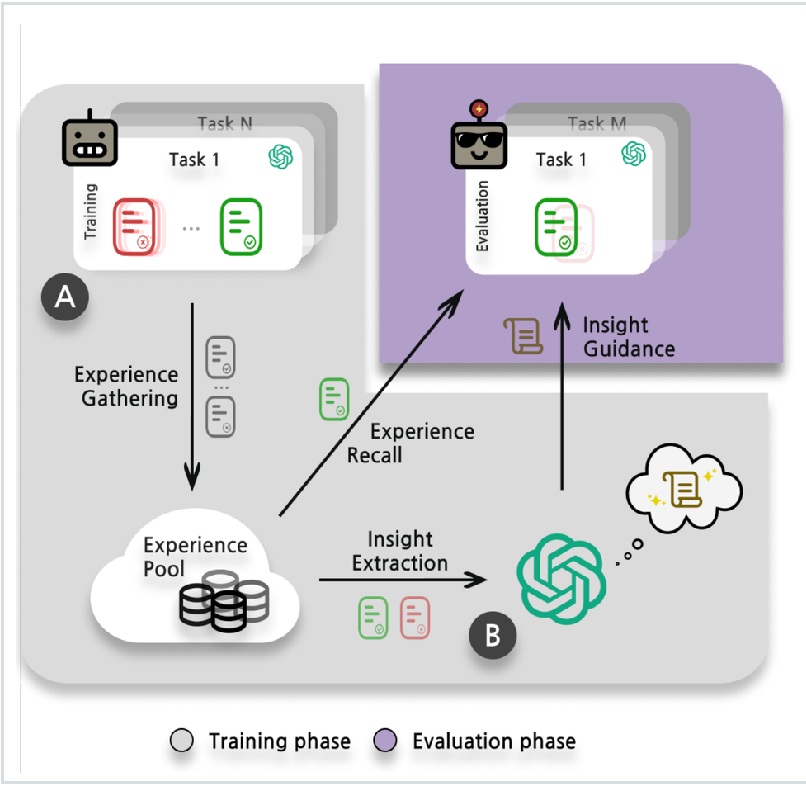
\includegraphics[width=0.72\textwidth]{figures/l4_expel_recall_insight_paths.pdf}
\caption{ExpeL从经验池走出两条路径：成功轨迹的经验回忆，以及比较经验后提取的洞见指导。官方课件第20页裁图，转引原论文图；相关口述：00:41:34--00:42:37。}
\label{fig:l4-expel}
\end{figure}

图\ref{fig:l4-expel}尤其值得仔细读。ExpeL（Zhao等，AAAI 2024）的经验池包含成功与失败；\textbf{取回作为few-shot示例的是成功轨迹}。失败与成功的配对比较、以及多条成功轨迹的共同规律，则用于\textbf{提取洞见（insights）}，形成另一条指导路径。课件的“保存成功与失败”概括了这类方法的经验来源，不能据此推断 ExpeL 把未加工的失败轨迹也当作成功示范塞给执行者。

\textbf{课堂问答：轨迹究竟是什么，检索是否要比较动作序列？}（00:42:37--00:44:01）讲者把轨迹解释为观察、动作和消息的连续记录；可以近似看作一次任务在上下文中发生的消息序列。对于检索，通常先嵌入\textbf{任务描述}，查找具有相似描述的旧任务，再取其关联轨迹，也可以限制为同一领域。课堂没有要求对动作序列做逐项比对，具体检索器仍是可以研究和替换的组成部分。

\begin{warningbox}{“相似经历”必须与“可执行指导”衔接}
过去成功不保证现在仍成功。任务文字可能接近，但网站、工具接口或约束已改变；原样示例还会携带当时的具体参数与冗余步骤。全轨迹检索提供了跨任务学习的基础，也引出下一章的问题：能否从轨迹中进一步提取范围明确、可复用的子过程？
\end{warningbox}

\subsection{本章小结}

MemGPT提供模型控制读写的数据通路；Mem0在写入前协调候选事实与已有事实；Reflexion把结果反馈转化为同一任务重试时可读的指导；相似轨迹检索则为新任务提供过去的行动示例。ExpeL还把成功与失败用于提炼一般洞见。它们共同说明，外部经验只有经过选择、解释并重新进入当前决策过程，才会影响智能体的行动。

\subsection{拓展阅读}

\begin{itemize}
\item \href{https://arxiv.org/abs/2310.08560}{MemGPT}、\href{https://arxiv.org/abs/2504.19413}{Mem0}：分别阅读记忆层级控制与事实更新机制。
\item \href{https://arxiv.org/abs/2303.11366}{Reflexion}、\href{https://arxiv.org/abs/2308.10144}{ExpeL}：分别阅读同任务反思与跨任务经验回忆／洞见提取。
\end{itemize}


\clearpage
\section{从一次经历到可复用技能：归纳与生命周期}

\subsection{技能的边界：寻找任务之间可重复的那一段}
前一章把过去的完整经历取回来，让模型参考一条已经走通的路线。接下来，Daniel Fried 把问题推进一步：如果两个任务只共享其中一段流程，能否把这一段单独提炼出来，让它成为之后随时可用的能力？这一转变决定了记忆保存的粒度。

例如，“搜索无线键盘”和“告诉我无线键盘的价格区间”都需要先找到搜索框、输入查询并提交。第二个任务还需要阅读结果中的价格、找到最低与最高价格，并向用户报告。若把整个价格查询任务保存下来，未来只想搜索商品的任务便会收到一些无关步骤；若把共同的搜索过程保存成技能，它就能服务于价格查询、加入愿望清单、加入购物车等多个目标。

\begin{importantbox}{本段核心定义：技能是可跨任务复用的子任务}
技能描述一块有明确用途的行为：输入是什么、应从何种状态开始、执行哪些操作、完成后得到什么。它可以是文本指导，也可以是可执行程序。技能归纳就是从具体任务经历中发现这种重复结构，并决定哪些细节应该保留、哪些应该变成参数。
\end{importantbox}

\begin{figure}[H]
\centering
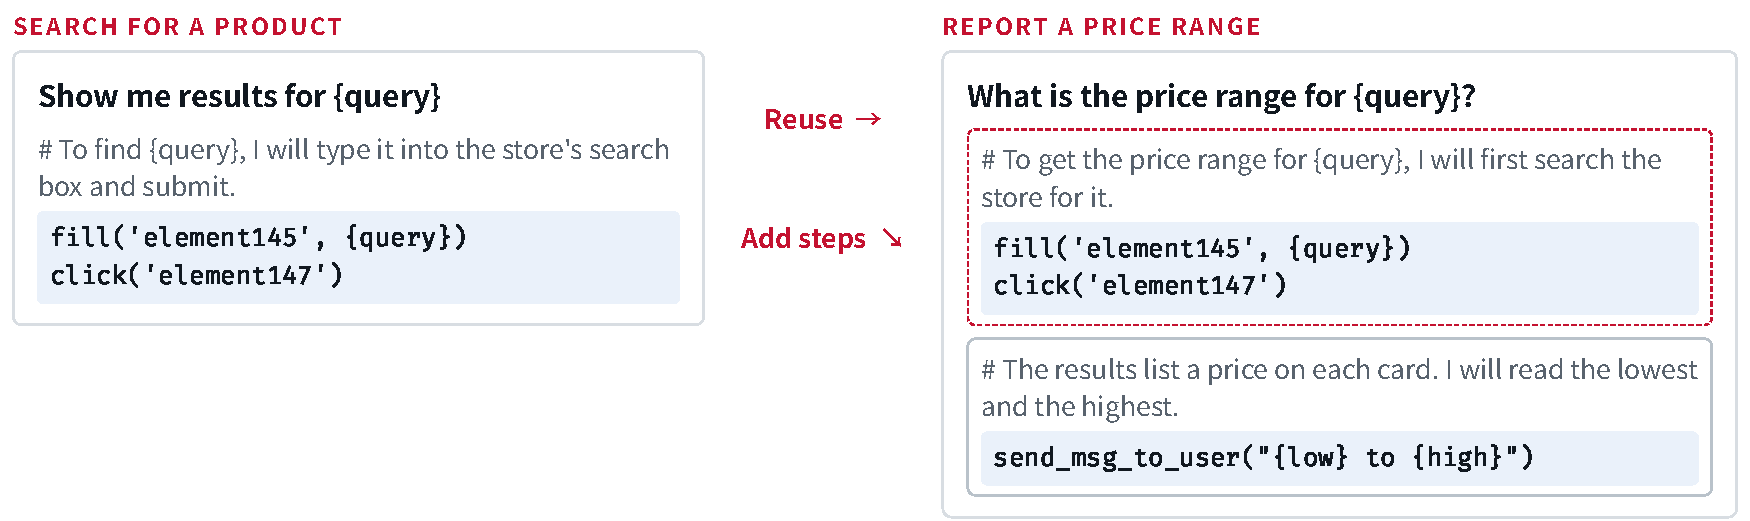
\includegraphics[width=\linewidth]{figures/skill_reusable_search_and_price_range.pdf}
\caption{搜索子任务可以在价格区间任务中复用，再接上读取价格和报告结果的步骤。官方课件第22页矢量裁图；对应口述00:44:01--00:46:31，非视频帧。}
\label{fig:l4-reusable-chunk}
\end{figure}

图\ref{fig:l4-reusable-chunk}同时暴露了抽象的局限。把查询文本变成 \texttt{query} 参数，只解决“下次搜索另一种商品”的变化；\texttt{element145} 和 \texttt{element147} 仍绑定了当时的页面。元素重新编号，或者另一个网站改用不同的搜索入口，流程便可能失效。学生在课堂上指出了这一问题，讲者也明确认可：\textbf{可复用的任务语义，并不自动保证底层动作能跨页面复用。}

这给技能设计留下两个独立问题。一是“这一段行为的职责是什么”，例如搜索商品；二是“这一段行为如何落到当前环境”，例如选择哪个搜索框、按回车还是点击按钮。前者适合保持稳定，后者常常需要重新定位或适配。后面的文本、代码与多态接口方案，都在安排这两部分的关系。

\subsection{历史脉络：把已有解法变成下一轮的积木}
课堂在00:46:31--00:48:07简要介绍 Voyager 与程序归纳研究。官方课件第23页还列出 DreamCoder、Stitch、LAPS 和 LILO。它们的共同思想是：解完一批问题后，不仅保留答案，还要总结其中反复出现的结构，扩充以后构造解法的基本积木。下面对五项工作作机制归纳，其中后三项的细节属于\textbf{课件与原论文补充}，讲者没有逐项展开。

\begin{figure}[H]
\centering
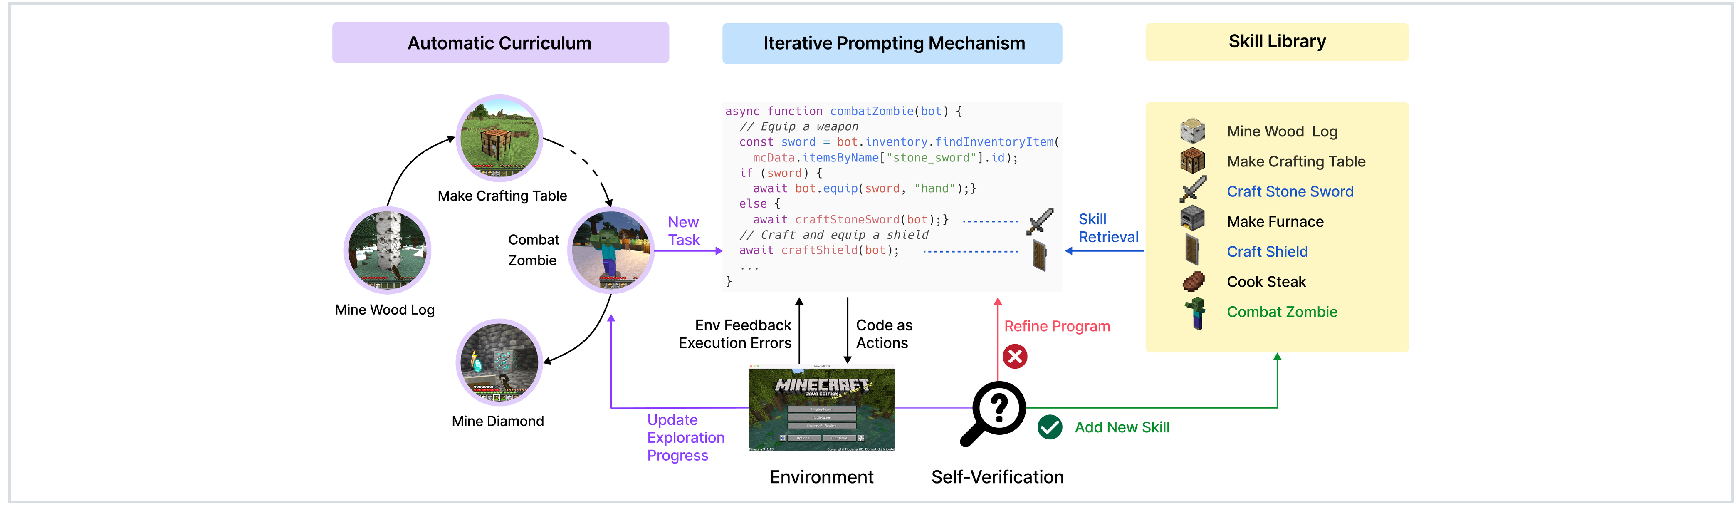
\includegraphics[width=\linewidth]{figures/voyager_curriculum_program_and_skill_library.pdf}
\caption{Voyager把自动课程、环境反馈驱动的程序修订和持续增长的技能库连成闭环。官方课件第23页矢量裁图；对应口述00:46:31--00:47:26，非视频帧。}
\label{fig:l4-voyager}
\end{figure}

\textbf{Voyager：在交互中长出函数库。}Minecraft 中的任务具有依赖关系：获取木头、制作工作台、制作工具，然后才能完成更复杂的采集或战斗任务。Voyager用代码控制行为，通过环境反馈、执行错误与自我验证反复修改程序；成功的程序进入技能库，后续程序可以调用它们。图\ref{fig:l4-voyager}中的战斗程序会调用已经学会的制作武器、制作盾牌等能力。学习在环境探索过程中持续发生，技能组合也随探索扩展。\footnote{原始来源：\href{https://arxiv.org/abs/2305.16291}{Voyager: An Open-Ended Embodied Agent with Large Language Models}。}

\textbf{DreamCoder：从已求解程序中发现可复用函数。}它反复交替进行两类工作：利用当前函数库搜索能解决任务的程序，再从这些程序中提炼新的抽象，同时改进指导搜索的神经模型。原本反复写出的低层结构，变成一个较短的函数调用；新抽象进入下一轮搜索语言，因而改变未来问题可以怎样被表达和求解。这里的核心是程序语料上的库学习循环，并非让浏览器 agent 在评价任务之间存入网页操作。\footnote{原始来源：\href{https://arxiv.org/abs/2006.08381}{DreamCoder: Growing Generalizable, Interpretable Knowledge with Wake-Sleep Bayesian Program Learning}。}

\textbf{Stitch：用符号压缩发现共享结构。}它接收一批程序，从基础语言构造候选抽象，利用程序中的结构匹配来缩减搜索范围，寻找能有效压缩语料的库函数。它主要承担“从现成程序中发现共用结构”的角色；环境探索、任务成功判定和自然语言命名，需要由其他模块提供。\footnote{原始来源：\href{https://arxiv.org/abs/2211.16605}{Top-Down Synthesis for Library Learning}，Stitch。}

\textbf{LAPS：让任务语言参与抽象和搜索。}自然语言标注可以提示哪些行为具有共同含义，也能帮助搜索模型优先探索更可能符合目标的程序。LAPS把语言信息接入库学习和程序搜索；它并不等同于让现代聊天模型把网页轨迹总结成一段文字。\footnote{原始来源：\href{https://arxiv.org/abs/2106.11053}{Leveraging Language to Learn Program Abstractions and Search Heuristics}。}

\textbf{LILO：生成、压缩、命名与文档相互配合。}LLM先参与产生解决问题的程序，Stitch再发现可复用函数，随后LLM根据用法为函数命名、生成文档。这些名称和说明会帮助下一轮程序生成理解新函数的用途。它说明了代码结构与自然语言说明可以共同组成技能库。\footnote{原始来源：\href{https://arxiv.org/abs/2310.19791}{LILO: Learning Interpretable Libraries by Compressing and Documenting Code}。}

\begin{knowledgebox}{“在线”和“离线”要看学习发生在哪个任务边界}
Voyager在环境交互中不断扩充技能库。DreamCoder及其相关库学习方法，主要从当前已经收集或求解出的程序集合中提炼抽象，并在下一轮搜索中复用；它们也可以迭代，但这不等于本课随后采用的在线网页评测。区分设置时，应说明数据来自哪里、何时更新技能库，以及更新后影响哪些任务，不能把“反复执行学习循环”直接称作在线测试。
\end{knowledgebox}

\subsection{在线评价：系统会带着先前任务的经验继续往前走}
现实用户可能连续提出一串相关任务。第一次让 agent 把一副 Sony 蓝牙耳机加入愿望清单，后面再查询新上架的游戏配件，最后问无线键盘的价格区间。完成第一项任务后，系统可能已经掌握“搜索商品”和“加入愿望清单”；后面的任务可以使用这些能力，甚至在它们上面构建更大的工作流。

\begin{figure}[H]
\centering
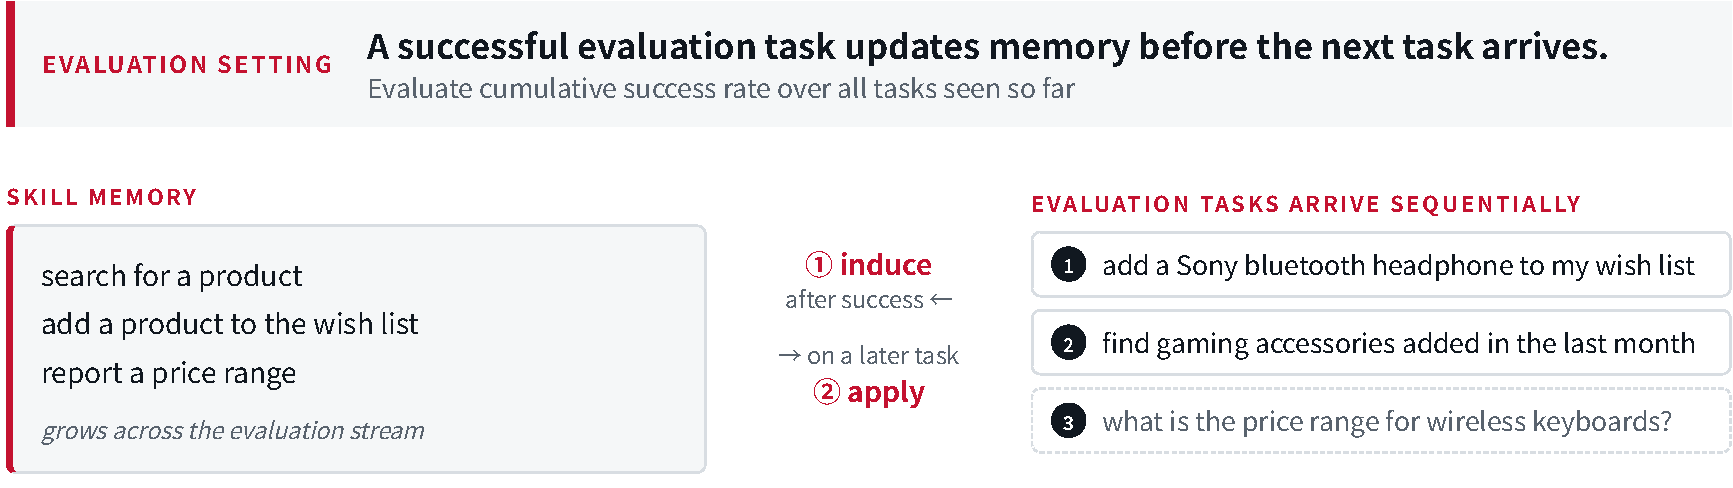
\includegraphics[width=\linewidth]{figures/online_evaluation_stream_and_growing_skill_memory.pdf}
\caption{评价任务依次到来，成功经历产生的技能在之后的任务中继续可用。官方课件第24页矢量裁图；对应口述00:48:07--00:50:11，非视频帧。}
\label{fig:l4-online-stream}
\end{figure}

这类评价允许\textbf{跨评价任务积累记忆}。一个任务执行完毕，系统判断结果、归纳技能并更新记忆，随后再处理下一个任务。它与“每道题都从相同的空记忆或固定技能库开始”的固定评测回答不同问题：前者测量连续使用后能否适应任务流，后者测量给定配置的能力。两者都合理，但比较结果时必须公开记忆是否更新、任务顺序和起始记忆。

图\ref{fig:l4-online-stream}提到的累计成功率，可以理解为：到当前时刻为止，已经看到的所有任务中，成功任务占多大比例。它把每个任务只计一次，不会因为之后学会了技能就自动改写先前的失败记录。为了把这个统计口径写清楚，可用以下教学公式表示：
$$
\operatorname{CSR}(n)=\frac{1}{n}\sum_{i=1}^{n}\mathbf{1}\{\text{第 }i\text{ 个任务成功}\}.
$$
\begin{itemize}
\item $n$：目前已经执行的任务总数。
\item $i$：按到达顺序编号的任务索引。
\item $\operatorname{CSR}(n)$：前$n$个任务的累计成功率。
\item $\mathbf{1}\{\cdot\}$：指示函数，括号内条件成立时取1，否则取0。
\item $\sum_{i=1}^{n}$：把前$n$个任务的成功指示值相加。
\end{itemize}

\begin{warningbox}{在线曲线上升，不代表每个后续任务都更容易成功}
累计曲线同时受到技能积累、任务难度和任务顺序影响；新增一个困难任务，也可能让累计成功率下降。要判断技能积累的作用，应在相同任务流、相同基础模型与相同评价规则下设置对照。尤其不能把在线适应的结果直接当成固定技能库在独立测试集上的成绩。
\end{warningbox}

\subsection{Learn、Use、Maintain：记忆是一种持续管理的资源}
技能库一旦能跨任务留存，就需要管理其整个生命周期。课件用三条链条概括后续研究：\textbf{Learn}决定学进来什么，\textbf{Use}决定此刻用什么，\textbf{Maintain}决定经验变化后保留、修复或淘汰什么。

\begin{figure}[H]
\centering
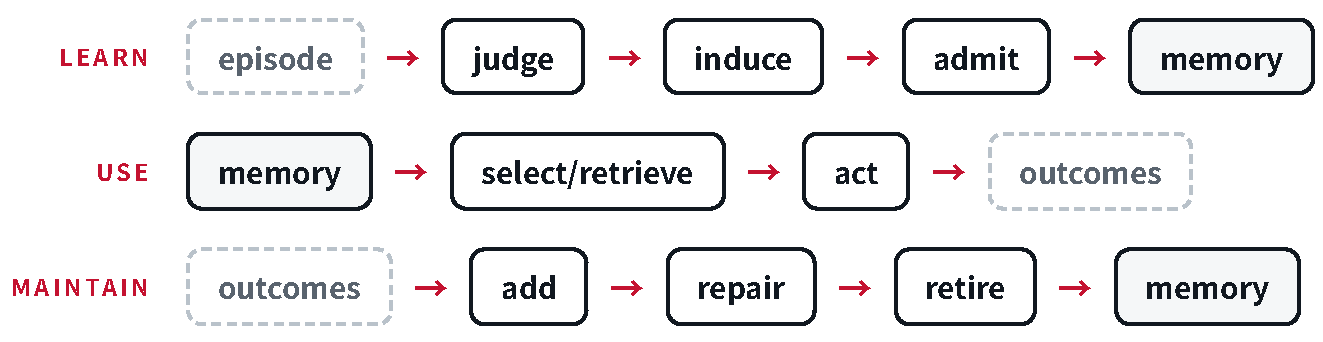
\includegraphics[width=\linewidth]{figures/skill_learn_use_maintain_lifecycle.pdf}
\caption{技能生命周期的三个环节：学习、使用与维护。官方课件第25页矢量裁图；对应口述00:50:11--00:51:14，非视频帧。}
\label{fig:l4-lifecycle}
\end{figure}

在\textbf{学习}阶段，一次任务经历提供候选证据。judge先判断经历是否可信，induce从中产生抽象，admit决定候选是否达到入库要求。它们承担不同职责：完成过任务不保证抽象后的技能仍正确，抽象得像一个技能也不保证值得存入记忆。

在\textbf{使用}阶段，系统从记忆中选择或检索相关技能，随后行动并观察结果。技能库里有一个函数，不等于模型一定会选对它；选对函数，也还需要满足它的起始状态和参数要求。

在\textbf{维护}阶段，实际使用结果反过来影响技能库。某个技能可能需要补充参数，另一个需要修复失效的页面操作，还有一些长期不用或高度重复的技能可以退役。课件列出的add、repair、retire是维护操作的类别，不要求每一次任务之后都严格按这三个操作顺序执行。讲者还提到概括过于具体的技能、合并重叠技能和清理无用技能，后文会进一步讨论。

\subsection{本章小结}
技能归纳从完整经历中找出可重复的子任务，并把具体解法变成以后的构造积木。历史工作分别突出环境探索、程序压缩、语言指导和可读文档。在线任务流使前一任务学到的技能可以帮助后一任务，因此评价必须说明记忆更新规则。Learn、Use、Maintain则提供一张统一地图：学到什么、如何调用、怎样修复与淘汰，都是系统能力的一部分。

\subsection{拓展阅读}
\begin{itemize}
\item \href{https://arxiv.org/abs/2305.16291}{Voyager}：观察环境反馈、自我验证与技能库怎样共同支持持续探索。
\item \href{https://arxiv.org/abs/2310.19791}{LILO}：理解程序压缩后，函数名称与文档为什么仍影响下一轮的使用效果。
\end{itemize}

\clearpage
\section{文本技能：Agent Workflow Memory怎样从轨迹归纳工作流}

\subsection{从“这次搜satisfied”到“以后搜任意评论词”}
Agent Workflow Memory（AWM）给技能归纳提供一个清楚的网页例子。用户问：店铺至今收到的评论里，有多少条提到了“satisfied”？agent进入Marketing菜单，打开All Reviews页面，在搜索框中输入该词，点击Search，然后读取结果并报告数量。

若只保存这次轨迹，记忆会含有特定查询词和特定答案。AWM希望从其中提炼“搜索包含某个词的评论”这一工作流，把具体的\texttt{satisfied}改成可替换的\texttt{term}。这样，下次用户问“disappointed”或“best”时，模型仍能利用同一流程。

\begin{figure}[H]
\centering
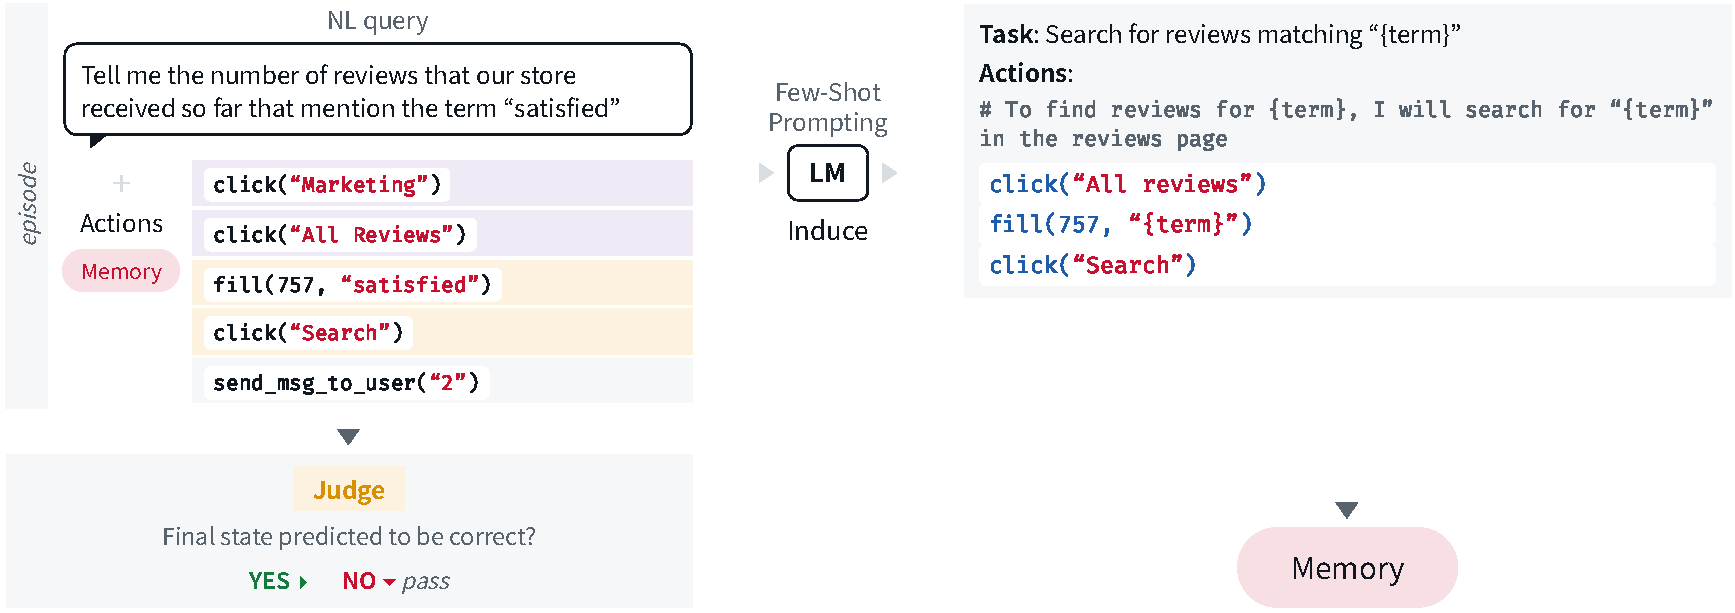
\includegraphics[width=\linewidth]{figures/awm_text_workflow_induction_and_judge.pdf}
\caption{AWM把任务与动作序列归纳成带参数的文本工作流，并根据judge对原经历的判断决定是否保存。官方课件第26页矢量裁图；对应口述00:51:14--00:54:20，非视频帧。}
\label{fig:l4-awm-induction}
\end{figure}

AWM的工作流包含两类信息。\textbf{任务描述}告诉模型这段流程的目标；\textbf{动作示例}告诉模型怎样在网页上实现这个目标。虽然示例包含\texttt{click}和\texttt{fill}，这里保存的整体仍是给模型阅读的文本模板。模型在新任务中需要重新观察页面、理解模板、填入参数并逐步输出动作；它没有自动获得一个能够一次执行全部步骤的新工具。

\begin{importantbox}{文本工作流的抽象发生在“固定部分与变化部分”的分界}
评论搜索中的目标词会变化，因此适合改成参数；“进入评论页、填写查询、点击搜索”是可重复的程序结构，因此适合保留。归纳的质量取决于能否找对这一分界。只替换一个词而保留所有偶然的页面细节，得到的仍可能是非常狭窄的模板。
\end{importantbox}

\subsection{judge、induce与admit各解决什么问题}
\textbf{judge解决证据质量问题。}模型可能走错页面、看错计数，或者没有完成用户要求。如果不做筛选，这些行为也会被记入工作流，给未来任务提供错误示范。课堂介绍的AWM在线流程使用judge模型预测原任务轨迹是否正确，预测成功的经历才被用于扩充工作流记忆。

\textbf{induce解决可复用结构问题。}归纳模型读取任务和工具调用，识别有用子任务，生成其描述与参数化动作模板。归纳本身允许重新划分边界：一个完整任务可以产生多个工作流，一个流程也可以只覆盖原轨迹中的部分步骤。

\textbf{admit解决候选是否入库问题。}课堂的AWM示意图主要用原经历的成功判断作为保存依据，尚未像后面的代码方案那样，把新抽象重新执行一遍。应保留这一区别：\textbf{“原轨迹预测成功”提供了学习素材，不能直接证明“新归纳工作流在未来任务中必然正确”。}

记忆最终进入语言模型的上下文。讲者指出，可以根据技能数量与上下文长度，提供完整工作流，也可以先提供任务描述，再选择需要的内容。因而系统设计还要考虑“保存多少”和“本次展示多少”；库内技能数量与实际送入上下文的数量并不必须相同。

\subsection{课件补充：被课堂跳过的归纳提示词}
在00:54:20，Daniel Fried明确表示因时间关系跳过归纳prompt。以下规则来自\textbf{官方课件第27页及AWM附录A.1}，用于帮助读者理解机制，不能记作讲者在口述中逐条讲解过的内容。

\begin{knowledgebox}{归纳prompt怎样约束“抽什么、抽多大、怎么写”}
提示词要求从网页任务及其动作序列中寻找反复使用的子流程，减少相似或重叠的工作流；每个工作流至少有两个步骤；变化的输入文本、按钮字符串等应以有说明力的变量名表示。这里的“两步”是这份提示词的设计约束，不能推广成所有技能的通用定义。\footnote{原始来源：\href{https://arxiv.org/abs/2409.07429}{Agent Workflow Memory}，附录A.1。}
\end{knowledgebox}

这些约束各有具体用途。要求至少两步，推动模型提炼有一定行为跨度的子流程；避免重叠，减少模型在用途相近的多个模板间选择的负担；用有说明力的变量名，则帮助未来调用者知道应替换什么。即使规则齐全，也仍需要判断抽出的流程是否过于依赖当前网页、是否把两个独立目标揉在一起，以及省掉的步骤是否其实是必要前置条件。

\subsection{跨任务复合：经验为什么能产生滚雪球效应}
AWM并不局限于每次重新发现一个独立小流程。先学会“按名称找到地点”，后面可以利用这个步骤查询地点邮编、查找附近咖啡馆或展示两地路线；再往后，任务可能要求“找到附近的Hilton酒店，并显示到附近超市的最短步行路径”。更复杂的任务需要重用此前已经接触过的子问题。

\begin{figure}[H]
\centering
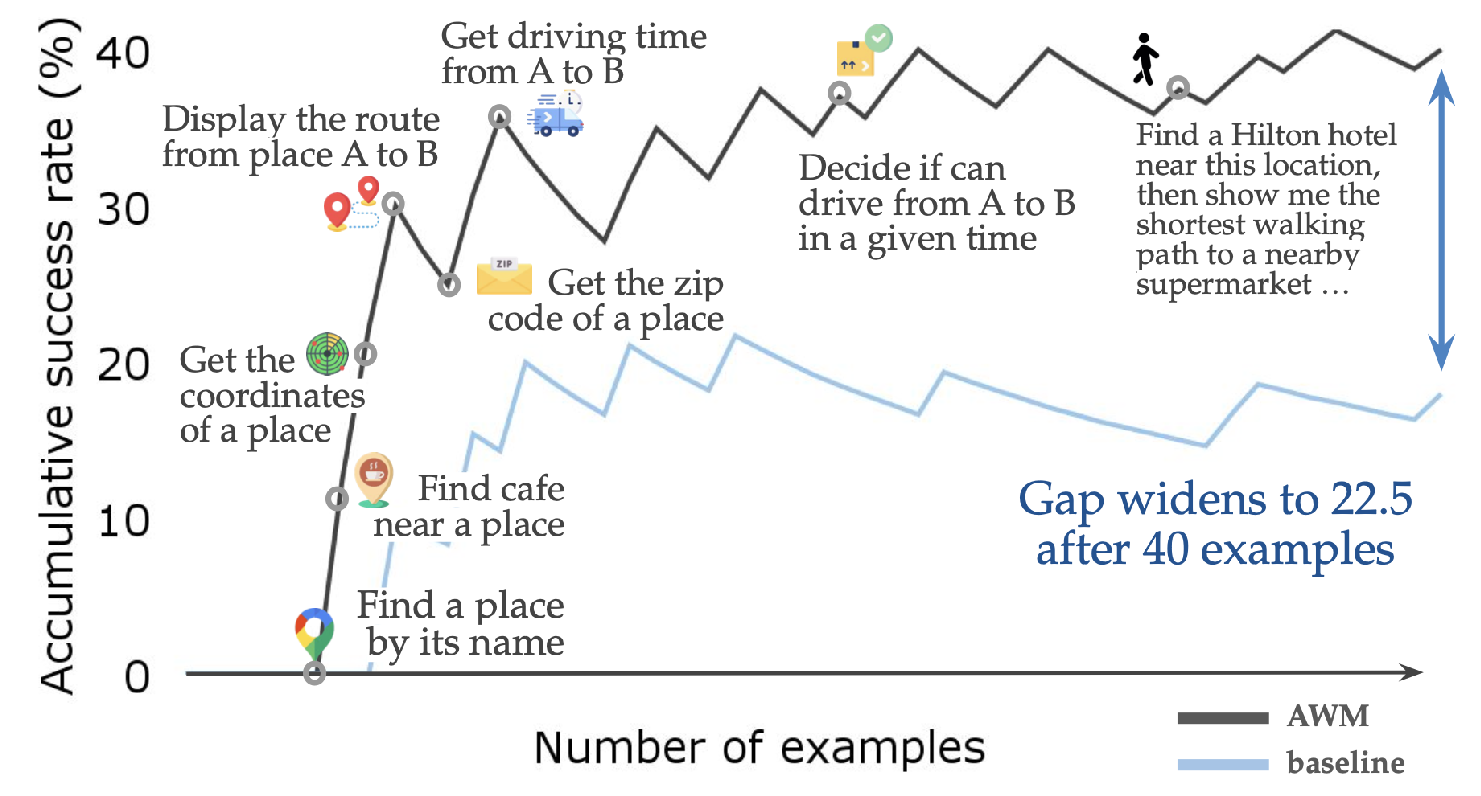
\includegraphics[width=\linewidth]{figures/awm_cumulative_success_and_compounding_tasks.pdf}
\caption{地图任务中，AWM的工作流记忆随任务流增长，累计成功率与基线拉开差距；图中标注40个样例后相差22.5个百分点。官方课件第28页矢量裁图；对应口述00:54:20--00:55:25，非视频帧。}
\label{fig:l4-awm-compounding}
\end{figure}

读图时先看坐标轴：横轴是已经处理的样例数量，纵轴是累计成功率。黑线为AWM，浅蓝线为不积累工作流的基线；文字标签说明在线过程中能够成功处理的任务种类。课件注明40个样例后差距达到22.5\textbf{个百分点}。这表达的是两个百分比的差值，不能写成相对提升22.5\%。

这张图的教学价值在于展示组合路径：简单操作有机会成为复杂流程的基础。它并不证明每条文字标签所示的任务都是被单一特定技能因果地解锁，也不能把单个地图任务流的差距视为所有网站的平均结果。口述中讲者用“约10\%”粗略形容基线；讲义采用图上明确标注的差值，不把这一口头近似当作图中终点的精确数值。

\subsection{文本与代码的分工：灵活性从哪里来，成本又留在哪里}
文本技能把一部分决策继续交给模型。当前网页搜索框的ID变了，模型可以根据新页面改用正确元素；旧流程少了一步，模型也可以临场补上。这种适应能力依赖模型正确解释技能，并结合观察作出选择。

同一特性也留下成本：模型仍要逐次产生低层动作。若一个流程包含“点击搜索框、输入查询、按回车”，文本模板可能帮助它更快想到这三步，但每一步仍可能消耗模型生成与观察。代码技能则能把这几个操作放进一个可执行函数，以一次技能调用启动整个流程。

\begin{warningbox}{“文本技能不提高效率”要理解到正确层面}
课件第36页用这句话概括文本技能没有直接把多个动作合成一次工具调用。它不意味着文本指导永远无法降低总步数：更好的指导也可能减少走错路和无关探索。后面的实验里，文本技能平均步数确实低于无记忆基线；代码技能进一步通过执行组合减少模型决策次数。
\end{warningbox}

\subsection{本章小结}
AWM把任务描述与动作轨迹整理成参数化文本工作流。judge提供原经历的质量筛选，induce负责发现子流程，admit决定保存候选；文本随后进入上下文，指导模型重新执行。其优势是模型可以根据当前页面调整步骤，局限是正确性仍依赖解释和逐步执行。工作流可以跨任务不断复合，但在线曲线的指标和任务流范围必须保留。

\subsection{拓展阅读}
\begin{itemize}
\item \href{https://arxiv.org/abs/2409.07429}{Agent Workflow Memory}：重点读工作流表示、在线与离线设置，以及附录A.1中的归纳提示词。
\item \href{https://arxiv.org/abs/2504.06821}{Inducing Programmatic Skills for Agentic Tasks}：沿着相同评论搜索例子，比较把技能放进文本记忆和注册为可执行动作的区别。
\end{itemize}

\clearpage
\section{可执行技能：验证、任务压缩与跨网站迁移}

\subsection{代码技能为什么同时改变动作空间和验证方式}
代码的关键价值是可以执行。若把“搜索商品”定义成函数，agent只需选择函数并传入参数，函数体就会完成若干底层操作。这个新函数还可以调用先前学会的技能，因此技能库能形成层次结构。

下面是官方课件第29页搜索函数的课程节选，省略了冗长的参数文档，保留实际操作。它依赖环境已提供的\texttt{click}、\texttt{fill}与\texttt{keyboard\_press}，不是一段可脱离浏览器环境独立运行的完整程序。

\par\noindent\begin{minipage}{\linewidth}
\begin{lstlisting}[language=Python,caption={课程节选：一次搜索技能调用执行三个低层操作（官方课件第29页，省略文档细节）}]
def search_product(search_box_id: str, query: str):
    """Search for a product using the given search box."""
    click(search_box_id)
    fill(search_box_id, query)
    keyboard_press('Enter')

search_product('595', 'Macbook')
\end{lstlisting}
\end{minipage}

执行时，三个低层动作仍然真实发生；省下的是模型在它们之间反复观察、决定与生成下一动作的过程。函数也会严格执行写在函数体里的步骤：如果当前网页必须点击一个按钮才能提交，而回车不起作用，函数需要修改。课堂学生用“rigid”概括这一局限。

\begin{importantbox}{代码技能的三个直接收益}
\textbf{可执行}：技能进入工具动作空间，模型可以直接调用。\textbf{可组合}：复杂技能调用简单技能，复用已有行为。\textbf{可测试}：存入技能库前运行候选程序，观察它能否在任务环境中达到目标。这些收益都要求代码和环境接口之间有真实、有效的连接。
\end{importantbox}

\subsection{ASI：先生成程序，再检验使用它的任务是否成功}
Agent Skill Induction（ASI）沿用任务经历归纳的入口，但把输出变成Python函数。评论检索例子被分成两个技能：\texttt{open\_marketing\_reviews()}负责进入评论区域；\texttt{search\_reviews(...)}负责按给定词执行搜索。前者保留站点内的菜单名称，后者将搜索框、搜索按钮和查询词作为参数；两个函数的泛化范围并不相同。

\begin{figure}[H]
\centering
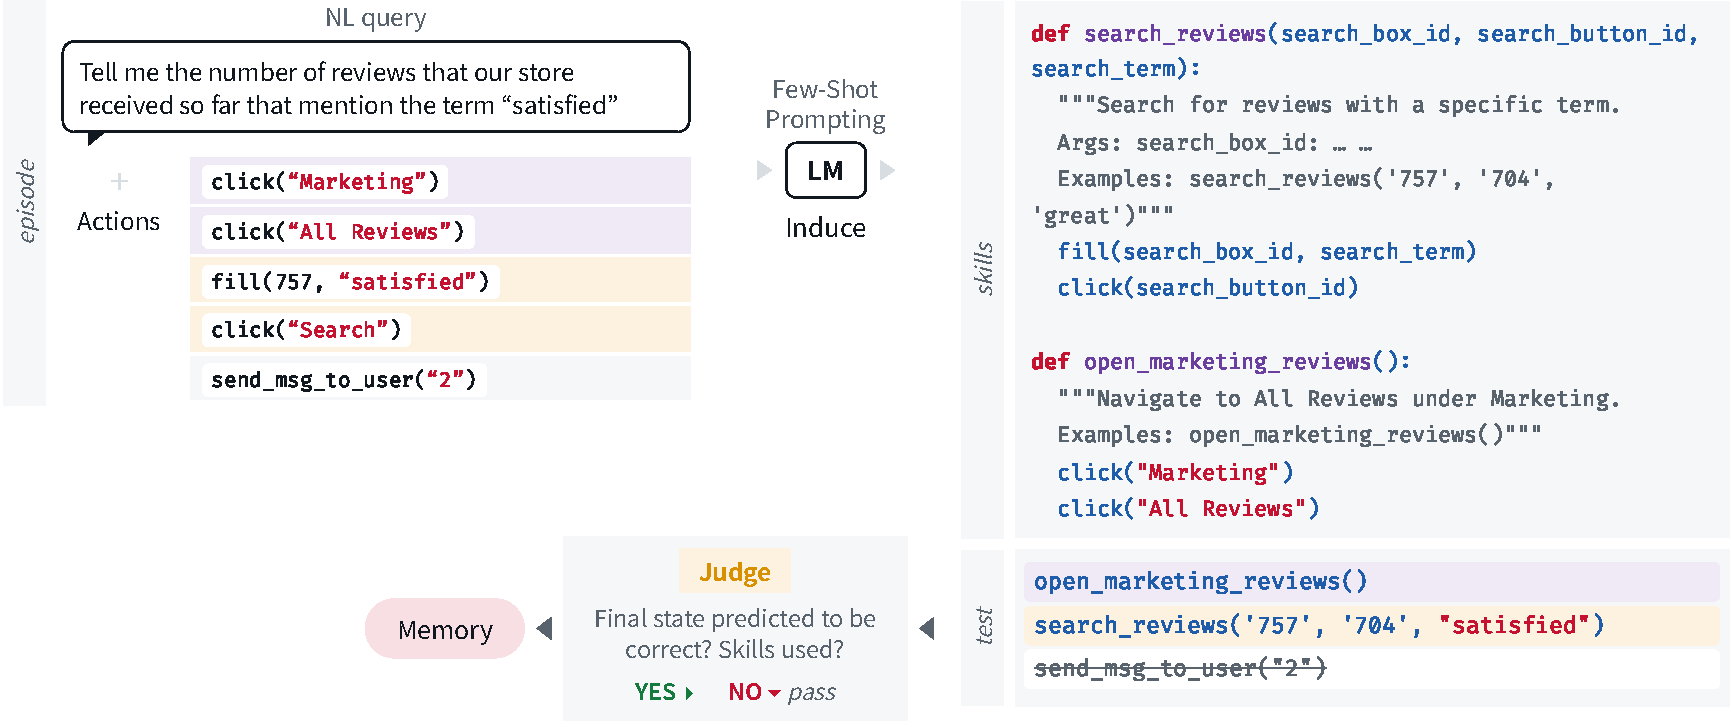
\includegraphics[width=\linewidth]{figures/asi_code_induction_rewritten_test_and_judge.pdf}
\caption{ASI生成代码技能后，将原轨迹改写为调用新技能的测试前缀，再检查执行结果。官方课件第30页矢量裁图；对应口述00:57:37--00:59:00，非视频帧。}
\label{fig:l4-asi-verify}
\end{figure}

验证的证据从“旧轨迹曾经成功”推进到“执行新抽象后，任务仍然成功”。ASI让归纳模型同时重写原始轨迹，把其中的低层动作片段替换成新技能调用，再在环境中执行。只有通过验证的技能进入库，随后作为新工具供模型使用。

\begin{knowledgebox}{原论文补充：防止“复制答案”造成虚假验证成功}
图\ref{fig:l4-asi-verify}把原来的\texttt{send\_msg\_to\_user("2")}划掉，是为了避免直接复制已知答案掩盖前面技能的失败。ASI删掉最后一次新技能调用之后的尾随原始动作，执行改写后的前缀，再让agent根据实际状态完成任务。论文还要求：最终任务预测正确、至少调用一个新技能，而且技能调用产生环境变化；入库的是实际调用过的技能。\footnote{原始来源：\href{https://arxiv.org/html/2504.06821v2}{ASI原论文}，第2.3节。此处具体检查规则是论文补充；课堂主要讲解执行后验证的思想。}
\end{knowledgebox}

这也是课件中judge旁“Skills used?”的含义。若把候选函数加入动作空间，然后只重跑同一个任务，模型可能继续使用旧有低层动作，完成任务却根本没试过新函数。这次成功不能证明新技能有效。因此，验证既要看任务结果，也要看候选技能是否真的参与了被测试的执行。

\begin{warningbox}{执行成功仍有适用范围}
在一个已知任务和已知网页上通过验证，提供的是该条件下的行为证据；它不会证明所有参数、所有起始页面或所有网站都正确。judge也只是一个模型判断器。应把验证理解为提高入库证据质量的方法，避免把它描述成无条件的正确性保证。
\end{warningbox}

\subsection{SkillWeaver：候选技能还能单独练习与修订}
当技能有了可执行代码，反馈就可以更细。任务级反馈告诉系统“目标有没有完成”；执行错误告诉系统“哪一行失败”；静态检查还能发现参数没有使用、代码结构可疑等问题。SkillWeaver通过实践、测试与修订，继续打磨候选技能。

课堂给出的例子是网页自动化函数\texttt{identify\_pill}。它接收药片刻印、颜色等参数；最初的版本虽然定义了\texttt{color}，函数体却没有使用它。结果是调用者传入\texttt{White}，搜索行为仍只按其他信息进行。这里讨论的是网页表单筛选的程序缺陷：\textbf{函数接口承诺接收的条件，没有落实到实际动作。}

\begin{figure}[H]
\centering
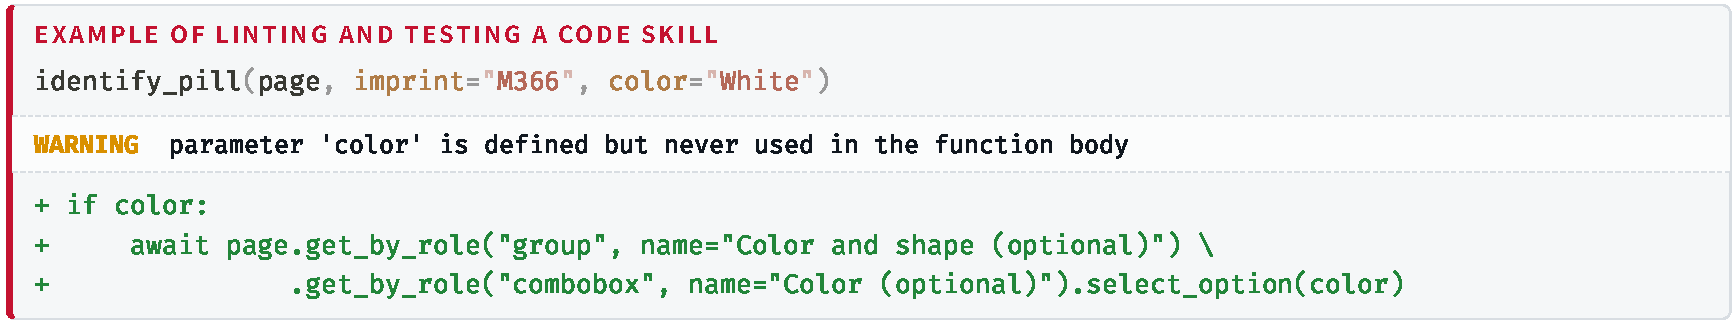
\includegraphics[width=\linewidth]{figures/skillweaver_unused_color_parameter_repair.pdf}
\caption{静态检查发现color参数未被使用，修订后函数按该参数选择颜色筛选项。官方课件第31页矢量裁图；对应口述00:59:00--01:01:02，非视频帧。}
\label{fig:l4-skillweaver-repair}
\end{figure}

修订在\texttt{color}有值时定位颜色选项并设置它，随后需要再次执行，检查目标页面状态。课堂还说明，可以把reward model对任务是否完成的判断作为修订反馈。静态检查和任务测试负责发现不同问题：前者容易定位“参数未使用”这样的结构缺陷；后者能验证页面是否真的接受输入、动作是否达到预期目标。

这种反馈循环把技能维护变成了具体动作：提出候选、实践、检查、修订、再次实践，通过后保存。它没有消除环境变化，但让变化后的问题能够在一段较小、可观察的代码里被处理。\footnote{原始来源：\href{https://arxiv.org/abs/2504.07079}{SkillWeaver: Web Agents Can Self-Improve by Discovering and Honing Skills}，API synthesis与skill honing部分。}

\subsection{任务压缩：减少的是模型决策步数}
更新账单地址与收货地址，看起来只是改两项资料，实际却需要进入账户设置、定位地址页面、填写多个字段并保存。每一步都要求模型重新读网页并决定下一动作时，冗余探索与重复推理会迅速累积。

\begin{figure}[H]
\centering
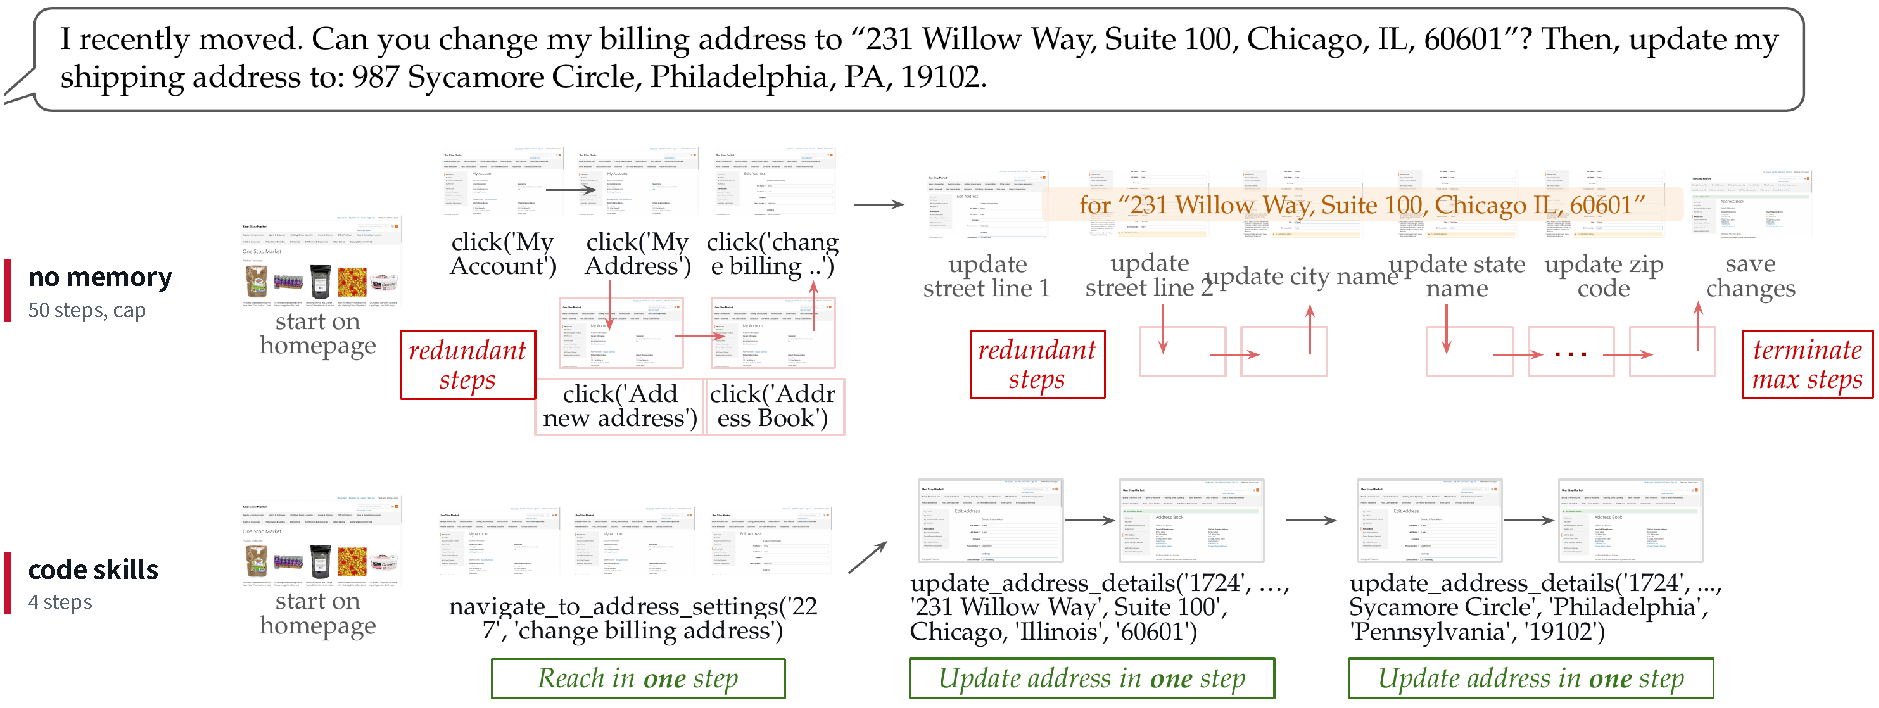
\includegraphics[width=\linewidth]{figures/asi_address_update_task_compression.pdf}
\caption{地址更新案例中，无记忆基线耗尽50步上限而未完成；代码技能版本用4个agent步骤完成。官方课件第32页矢量裁图；对应口述01:01:02--01:02:48，非视频帧。}
\label{fig:l4-task-compression}
\end{figure}

图\ref{fig:l4-task-compression}下方用“进入地址设置”和两次“更新地址明细”等技能，把多字段编辑压缩为少量高层决策。讲者口述强调三个主要技能调用，课件及论文对完整任务采用的计步结果是\textbf{4步}；讲义据此报告。上方的\textbf{50步是最大步数限制，并且该基线在上限处失败}，不能写成两个成功解法“从50步优化到4步”。

减少模型步数可能同时带来两类收益。第一，省去每个字段之间的模型调用、网页重观察和下一动作生成。第二，在高层技能之间规划，减少进入无关页面、忘记当前字段或误走重复路径的机会。网页内部仍要完成相应填表与点击；低层动作数量、模型动作数、token成本和实际运行时间，是相关但不同的指标。

\subsection{定量证据：检查点完成率与平均agent步骤}
课堂接下来比较无记忆、文本技能和代码技能。这里的任务被扩展成包含更多重复子任务的长流程，例如一次添加多件商品、检索多个查询词的评论数量，或连续修改若干信息。为了衡量部分完成，实验设置中间检查点。

\begin{figure}[H]
\centering
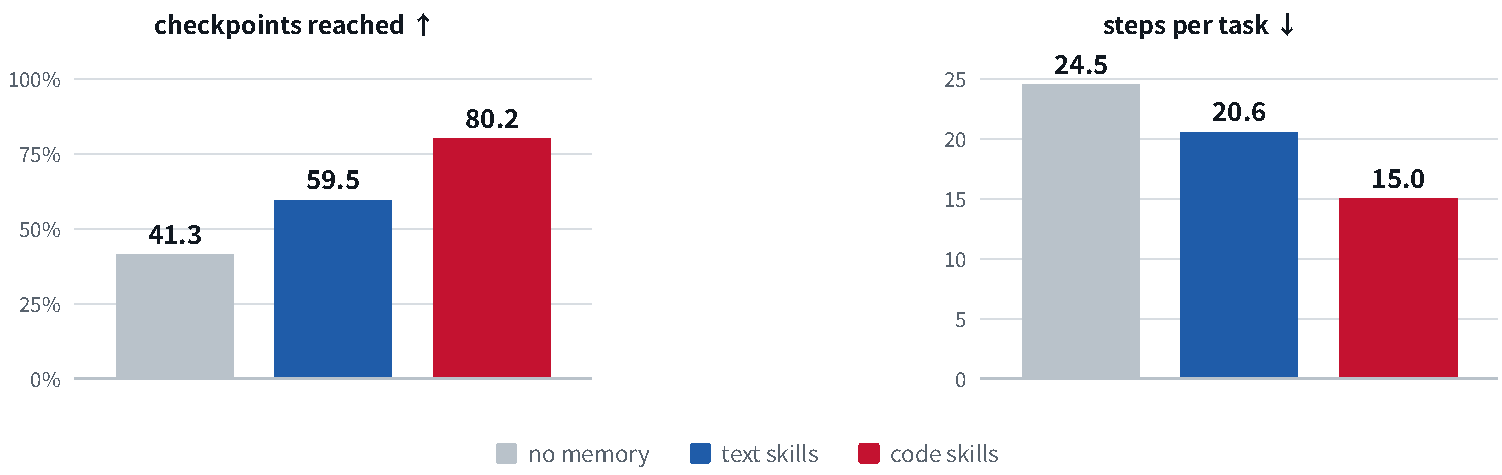
\includegraphics[width=\linewidth]{figures/asi_checkpoints_reached_and_agent_steps.pdf}
\caption{重复结构较多的扩展网页任务中，代码技能提高检查点完成率并减少agent步数。官方课件第33页矢量裁图；对应口述01:02:48--01:03:18，非视频帧。}
\label{fig:l4-asi-metrics}
\end{figure}

若任务要求把五件不同商品加入购物车，每件商品可以对应一个检查点；完成其中三件，便获得部分完成分数。为了明确这与“整道任务成功或失败”的二元判断不同，可写成以下教学公式：
$$
\operatorname{CheckpointRate}(q)=\frac{c_q}{C_q}\times100\%.
$$
\begin{itemize}
\item $q$：一个待完成的任务。
\item $C_q$：该任务预先规定的检查点总数。
\item $c_q$：agent实际达到的检查点数量。
\item $\operatorname{CheckpointRate}(q)$：该任务的检查点完成百分比。
\item $100\%$：将完成比例表示为百分数的换算因子。
\end{itemize}

\begin{center}
\begin{tabularx}{\linewidth}{lXX}
\toprule
表示方式 & 检查点完成率（越高越好） & 每任务agent步骤（越少越好）\\
\midrule
无记忆基线 & 41.3\% & 24.5\\
文本技能（AWM） & 59.5\% & 20.6\\
代码技能（ASI） & 80.2\% & 15.0\\
\bottomrule
\end{tabularx}
\end{center}

这些数值对应Shopping、Admin、Reddit、GitLab、Map五个WebArena站点上的\textbf{扩展任务实验}，是五个站点列结果的等权平均并按课件精度四舍五入。例如基线的检查点完成率由41.7、58.0、33.3、33.3、40.0平均得到41.3\%。它们不是WebArena全部812个常规任务的完整成功率。实验比较使用同一Claude 3.5 Sonnet基础模型和BrowserGym框架。\footnote{已核对\href{https://arxiv.org/pdf/2504.06821}{ASI的COLM 2025论文版本}第4节与表4（PDF第7页）。官方课件第33页将来源写成表2，但论文表2是技能示例表；本讲义按原论文校准为表4。}

\begin{importantbox}{这个对照支持的结论与边界}
在具有大量重复结构的扩展网页任务中，文本工作流改善了任务进展；可执行技能进一步提高检查点完成率，并减少模型需要作出的agent动作。它支持程序表示、执行验证与高层动作组合的整体方案，不能据此断言任何网站、任何任务分布上的代码技能都优于文本技能，也不能把80.2\%解释成完整任务成功率。
\end{importantbox}

\subsection{迁移失败：参数变化与交互结构变化不是同一种问题}
代码技能的脆弱性在跨网站时更明显。元素ID变化时，若技能把ID作为参数，调用者还有机会找到新ID再调用。但\textbf{交互结构变化}会使函数体本身不适用：旧网站使用下拉菜单，另一个网站使用侧栏中的单选按钮，即使能定位到排序入口，旧的\texttt{select\_option}动作也未必能完成选择。

\begin{figure}[H]
\centering
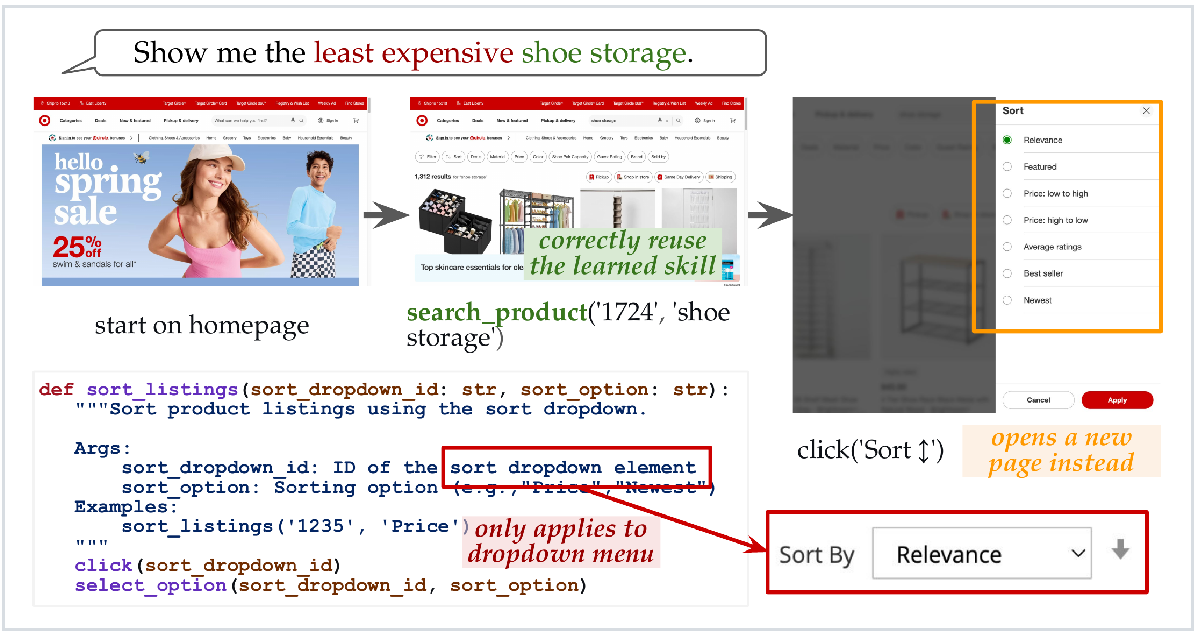
\includegraphics[width=0.96\linewidth]{figures/asi_sort_dropdown_to_target_sidebar_failure.pdf}
\caption{搜索商品技能可以复用，但sort\_listings假定下拉菜单，Target的排序界面却打开侧栏。官方课件第34页矢量裁图；对应口述01:03:18--01:04:20，非视频帧。}
\label{fig:l4-transfer-failure}
\end{figure}

图\ref{fig:l4-transfer-failure}中，agent先成功搜索shoe storage，接下来希望按价格排序。归纳自其他网站的\texttt{sort\_listings}接收下拉控件ID和排序选项，执行“点击控件、选择选项”。Target则先打开排序侧栏，再让用户选择一组按钮中的选项，最后应用。失败来自程序中固化的控件语义与新站点不匹配；重新填一个ID不能解决所有问题。

这把Maintain中的repair落实为两种常见工作：更新元素定位，或者更新实现流程。两者都需要当前环境的证据。某些技能可以在新站点继续使用，某些需要改写，还有一些可能应当暂时禁用；仅用函数名称相同来判断可迁移性是不够的。

\subsection{PolySkill：稳定接口之下，让每个网站提供自己的实现}
如果“搜索商品、加入购物车、开始结账”的目标在多个购物网站都存在，就可以将这些目标定义成共有接口；不同网站用各自的操作实现接口。复合任务则调用这些接口，减少对某一种具体界面动作的依赖。这是PolySkill引入多态抽象的动机。

\begin{figure}[H]
\centering
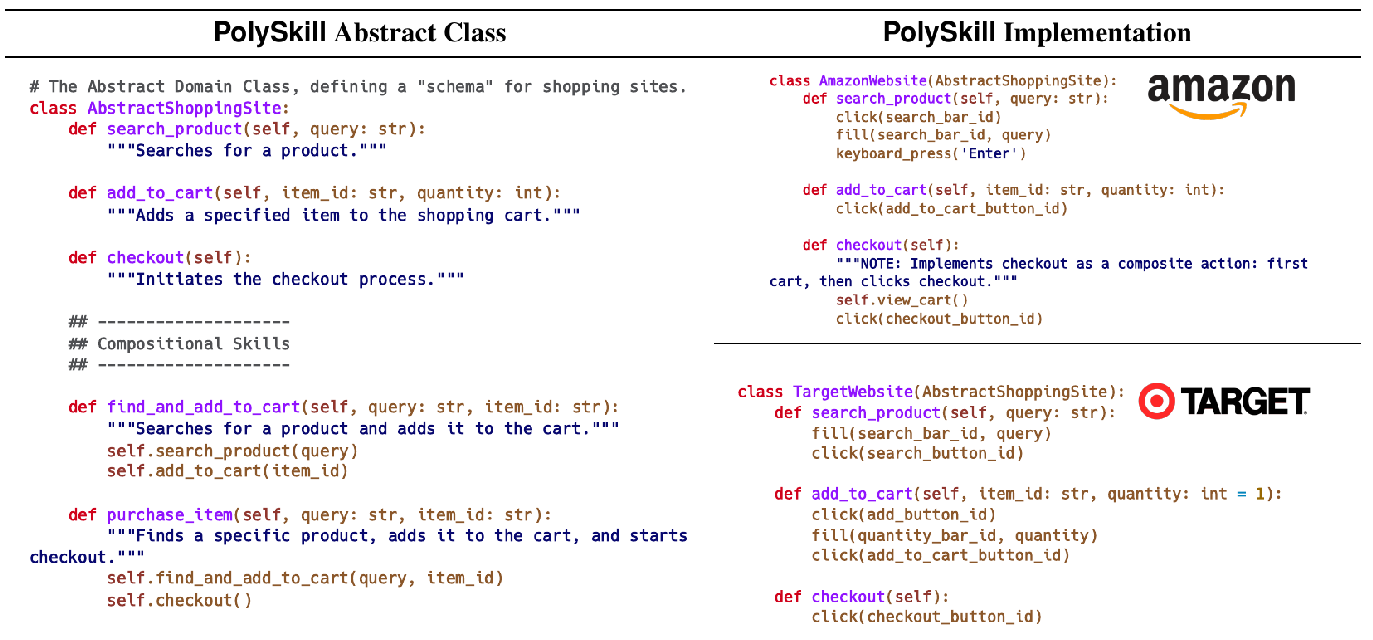
\includegraphics[width=\linewidth]{figures/polyskill_abstract_interface_and_site_implementations.pdf}
\caption{PolySkill的抽象购物接口与Amazon、Target实现：复合技能调用共有方法，具体方法决定页面动作。官方课件第35页矢量裁图；对应口述01:04:20--01:05:35，非视频帧。}
\label{fig:l4-polyskill}
\end{figure}

读图\ref{fig:l4-polyskill}时，可以沿两个方向看。左侧先定义\texttt{search\_product}、\texttt{add\_to\_cart}和\texttt{checkout}的用途。

基础方法再组合成更大的技能：\texttt{find\_and\_add\_to\_cart}负责搜索并加购商品；\texttt{purchase\_item}进一步调用结账。复合技能调用\texttt{self.search\_product(...)}等接口，因此不需要直接写某个网站的搜索框ID。

右侧则为每个网站填写实现。Amazon示例把查询填入搜索框后按回车；Target示例填入查询后点击搜索按钮。加入购物车的步骤也不同：Target实现还包含填写数量等动作。上层流程仍能用共同的“搜索、加购、结账”顺序，而低层细节由当前网站的实现承担。

讲者介绍的学习过程是：第一次进入一种网站类别时，建立抽象类与方法用途；在具体站点上，从成功经历归纳符合接口的实现。之后访问另一个站点，可以保留该类别的接口，学习新的实现。根据站点元数据或模型对当前环境的判断，只激活适用的实现，也能减少把大量无关技能同时提供给模型的问题。\footnote{原始来源：\href{https://arxiv.org/pdf/2510.15863}{PolySkill: Learning Generalizable Skills Through Polymorphic Abstraction}，表1。已对照原论文表格检查课件中的接口与两站点实现。}

\begin{knowledgebox}{接口抽象的边界：语义共用，执行证据仍需本地获得}
一个共有接口让复合流程可以复用，却不会自动找出新网页的按钮和表单。网站实现仍要通过交互与验证获得。表1是结构示意，省略了部分对象状态、元素定位及参数约定；不能将图中的代码直接当成可运行的完整类库。真实实现还需要让方法签名、默认参数、前置状态与返回结果彼此一致。
\end{knowledgebox}

这里的抽象承担了真实的环境边界：它把同一任务职责映射到多种站点操作，并让复合行为依赖稳定职责。

\subsection{把三种表示放在同一张决策地图上}
课件第36页用完整经历、文本技能和代码技能概括本段。完整经历保存具体行为，细节丰富但通常较长，迁移时需要识别哪些步骤还能用。文本技能压缩出有目的的子流程，模型在当前页面解释并调整它；代价是低层动作仍由模型逐步发出。代码技能把流程固定为可执行行为，便于调用、组合和测试；环境发生结构变化时，也更需要定位与修订。

\begin{importantbox}{表示选择决定“模型继续决定多少，工件固定执行多少”}
希望在新页面上保留临场调整空间，可以让文本提供策略与约束；希望重复流程快速、稳定地执行，可以用代码承担已经验证的行为。两者可以组合：文本说明什么时候使用、需要哪些前置条件，代码负责怎样执行，维护机制负责发现失效并修复。组合方式本身仍是开放研究问题。
\end{importantbox}

\subsection{本章小结}
可执行技能同时增加了工具动作、测试对象和组合积木。ASI通过执行使用新技能的轨迹提高入库证据质量；SkillWeaver把静态检查与实践反馈用于修订；扩展任务实验展示了在重复结构较多时，高层调用带来的检查点与步数收益。跨网站失败说明固化控件假设会限制迁移。PolySkill用共有接口与站点实现保留上层组合，同时把环境差异交给具体实现和验证。

\subsection{拓展阅读}
\begin{itemize}
\item \href{https://arxiv.org/abs/2504.06821}{Inducing Programmatic Skills for Agentic Tasks}：重点核对第2.3节的验证流程与第4节的扩展任务指标。
\item \href{https://arxiv.org/abs/2510.15863}{PolySkill}：对照表1追踪抽象接口、站点方法和复合技能之间的调用关系。
\end{itemize}


\clearpage
\section{失败经验与技能库维护：让记忆持续有用}

前面的技能归纳过程主要从成功轨迹出发：先完成任务，再提取可复用的部分。这个顺序有明确的理由，成功的行为更适合充当示范。但一个长期工作的智能体还会积累大量失败、重复功能和逐渐失效的技能。只增加记忆，无法回答这些内容是否值得保留、应该怎样使用，以及何时应该退出技能库。本章沿着课件第37--42页讨论技能生命周期中的三个问题：从失败中学什么，怎样判断经验，以及怎样控制记忆的使用与规模。

\subsection{从一次搜索失败提炼预防策略}

ReasoningBank 提供了一个具体的购物案例。用户希望得到 Sony 蓝牙耳机的完整型号名称，以及可用型号的价格范围。智能体搜索 \texttt{Bluetooth headphones Sony}，却得到5,578条来自不同商品部门的结果，每页仅显示12条。讲者解释，这个网站的查询匹配行为近似把关键词按“或”连接，因而搜索结果包含大量仅满足部分词语的商品。智能体不断翻页，直到耗尽步数，最后没有向用户交付结果。

问题发生在搜索与浏览策略上。即使每一页的“下一页”按钮都能正确点击，约465页的结果也无法靠有限的交互预算逐页检查完。把这条失败轨迹原样保存，留下的是一段反复翻页的行动记录；要帮助下一次任务，归纳过程还需要找出让搜索失控的条件，以及可以替代它的操作。

\begin{figure}[H]
\centering
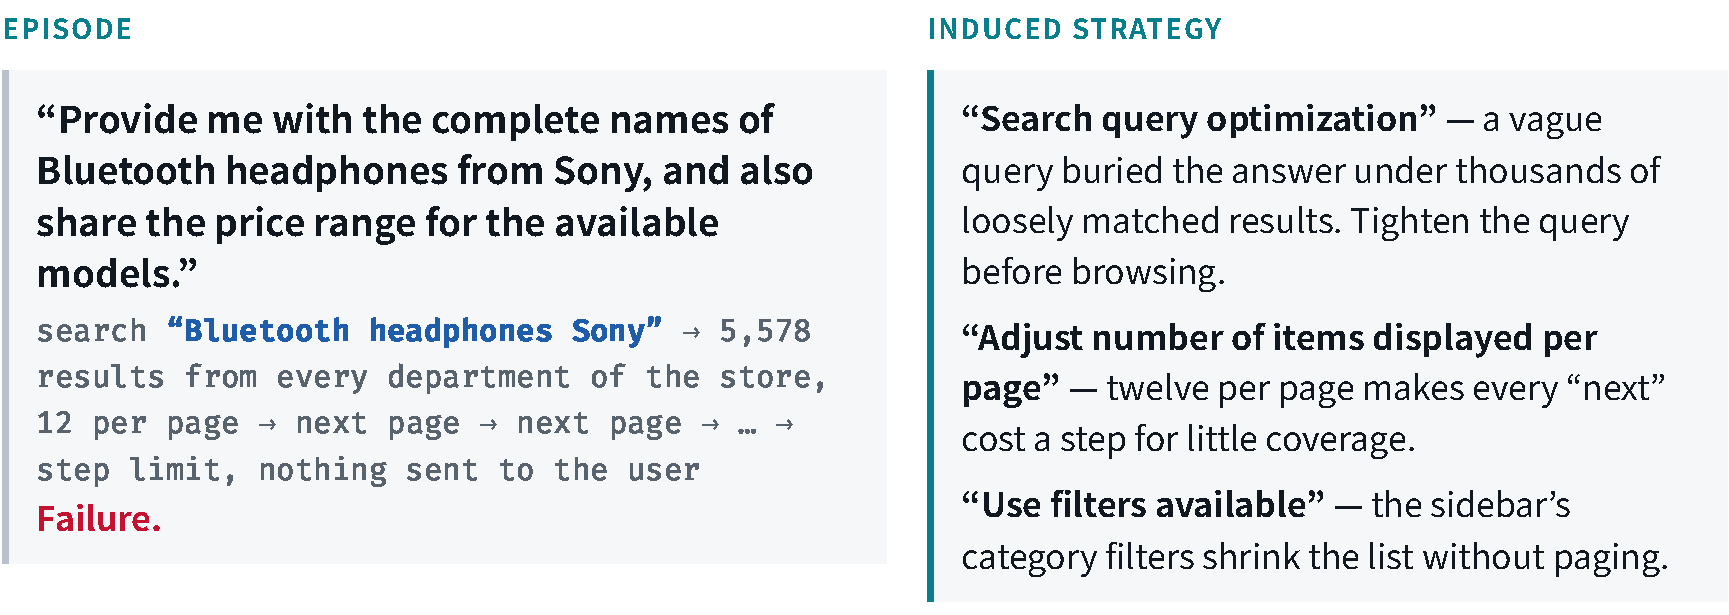
\includegraphics[width=\linewidth]{figures/failure_to_search_strategies.pdf}
\caption{搜索失败如何转化为预防策略。来源：官方课件第38页矢量裁图；相关口述区间01:06:22--01:08:50。图源为官方PDF，非视频截图。}
\label{fig:l4-failure-strategy}
\end{figure}

课件把这次失败提炼为三个策略。第一，收紧查询，先减少宽泛匹配；第二，调整每页显示数量，使一次观察覆盖更多候选商品；第三，利用侧栏中的类别筛选，在翻页之前缩小结果集合。这三个策略分别改变了候选集合、每步的信息量和筛选路径。它们保留了失败的原因与可采取的修正，并没有绑定到某一副耳机或某一个按钮编号。

这也说明了失败经验与成功示范在教学用途上的区别。成功轨迹可以示范“怎样做”；失败策略需要解释“在什么条件下会走错，以及应怎样预防”。后一种表达允许智能体在新任务里识别相似条件，再选择适当的动作。讲者把它与前面介绍的反思方法联系起来：让模型查看完整经历，说明失败原因，再把这些教训存到跨任务记忆中。

\begin{importantbox}{失败本身不自动成为有用技能}
一次失败提供的是证据。可复用的部分通常需要进一步归纳：指出触发失败的条件，解释失败机制，并给出能在未来任务中执行的调整。ReasoningBank 的案例把“不断翻页直到耗尽步数”转化为查询优化、扩大每页覆盖和使用过滤器。
\end{importantbox}

\subsection{为什么失败对不同记忆表示的作用不同}

课件比较了三种保存方式：Synapse 保存完整轨迹，AWM 保存从轨迹中抽出的工作流，ReasoningBank 保存文字策略。在 WebArena 的购物子集上，基座模型固定为 Gemini-2.5-Flash，再分别比较“只使用成功经验”与“加入失败经验”。图\ref{fig:l4-failure-memory}的纵轴是任务成功率，单位为百分比；它不是每一步的动作正确率，也不是记忆条目的正确率。

\begin{figure}[H]
\centering
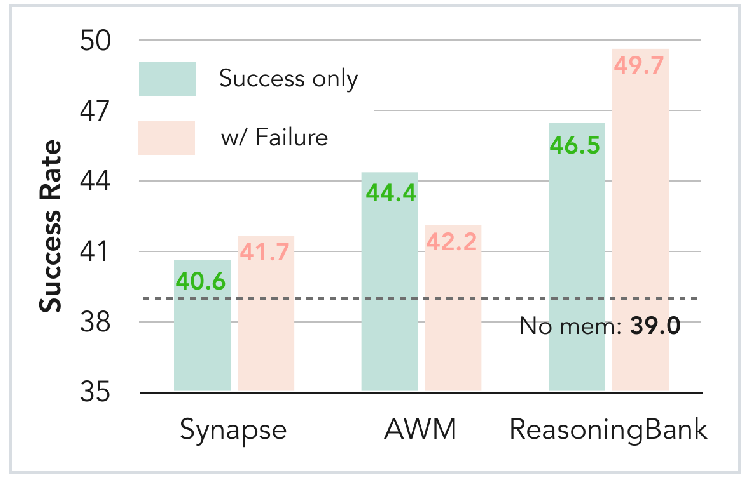
\includegraphics[width=0.70\linewidth]{figures/failure_memory_comparison.pdf}
\caption{失败经验的收益依赖记忆表示。来源：官方课件第39页矢量裁图；相关口述区间01:06:22--01:08:50。设置为 WebArena-Shopping、Gemini-2.5-Flash；图源为官方PDF，非视频截图。}
\label{fig:l4-failure-memory}
\end{figure}

无记忆基线为39.0\%。加入失败经验后，Synapse 从40.6\%略增到41.7\%，AWM 从44.4\%降到42.2\%，ReasoningBank 则从46.5\%提高到49.7\%。因此，准确的读法是：策略表示在这个实验中从失败获得了更明显的收益；轨迹表示的收益较小，工作流表示则出现下降。不能把图概括为“失败会让所有轨迹记忆变差”。

讲者给出的解释是，轨迹与工作流更接近行为示范。一个失败行动序列如果作为例子进入上下文，模型还需要额外辨别哪些动作不应该模仿。策略文字则可以直接说明怎样避免失误。不过，这是一种与案例相符的机制解释；图中并没有把“错误模仿”从其他因素中单独隔离出来。

\begin{warningbox}{保留失败轨迹与提炼失败教训是两个决策}
加入相同类型的原始经验，不保证不同记忆系统都会受益。归纳方式决定了经验进入上下文时扮演的角色：它可能是一段待模仿的行为，也可能是一条带条件的预防策略。上述结果支持在该模型和购物任务设置中使用失败策略，不能据此断言文字策略在所有任务中都优于工作流。
\end{warningbox}

\subsection{判定器不完美：校准实验测到了什么}

技能归纳常常依赖一个模型判定器：给它任务、执行轨迹和最终状态，让它判断任务是否成功。这个判断影响后续记忆的内容。误把失败当作成功，可能把错误动作当成示范；误把成功当作失败，又可能提炼出并不存在的问题。因此，判定质量会沿着“判断、归纳、存入”的链条影响后续任务。

ReasoningBank 的校准实验把判定器的准确率作为可控变量。实验先取得真实成功或失败标签，再以固定概率翻转标签：100\%准确率直接使用真值，90\%准确率意味着90\%的机会使用真值、10\%的机会使用相反标签，直到50\%这一二分类随机猜测水平。横轴表示\textbf{模拟判定准确率}，纵轴仍是后续智能体的\textbf{任务成功率}。

\begin{figure}[H]
\centering
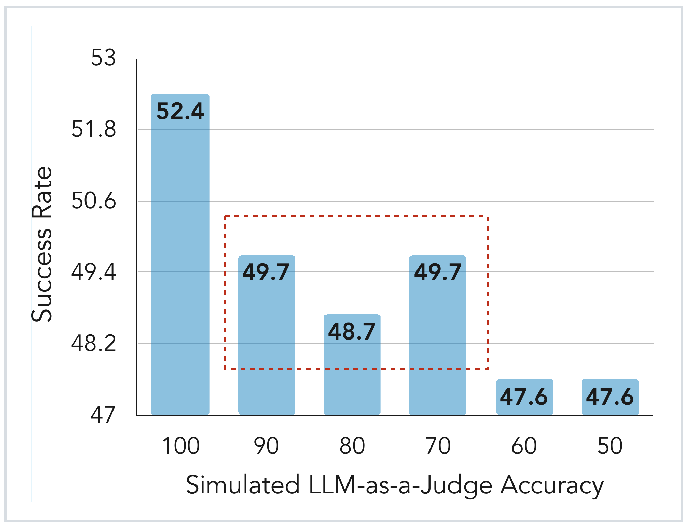
\includegraphics[width=0.67\linewidth]{figures/simulated_judge_accuracy.pdf}
\caption{通过真值标签翻转模拟判定噪声。来源：官方课件第40页矢量裁图；相关口述区间01:08:50--01:10:19。图源为官方PDF，非视频截图。}
\label{fig:l4-judge-calibration}
\end{figure}

使用真值判定时，成功率为52.4\%。模拟判定准确率为90\%、80\%、70\%时，对应成功率分别为49.7\%、48.7\%、49.7\%；降到60\%和50\%时，二者都为47.6\%。这组数值显示，在该设置中，70\%--90\%的模拟判定质量产生了相近的任务表现，而完美判定仍有优势。曲线也并非逐点单调，不能把几个实验点当成精确的函数关系。

\begin{warningbox}{模拟噪声不等于真实判定器的错误分布}
图中的90\%或70\%来自按概率翻转真实标签，不能读成某个真实模型的实测能力。真实判定器可能在某类任务上反复出错，错误也可能与轨迹长度、答案形式或环境状态相关；随机翻转实验没有证明系统同样能抵抗这些结构性错误。它提供的是受控噪声下的鲁棒性证据。
\end{warningbox}

\subsection{过量检索：更多经验为何可能妨碍行动}

正确经验也需要经过选择。ReasoningBank 的另一项消融固定 WebArena-Shopping 和 Gemini-2.5-Flash，改变每次检索的经验数量。无记忆时成功率为39.0\%，检索一条经验提高到49.7\%；检索二、三、四条时，成功率分别下降到46.0\%、45.5\%和44.4\%。图\ref{fig:l4-over-retrieval}的横轴是检索出来的\textbf{经验数量}，不是整个库的大小，也不是一次任务实际调用技能的次数。

\begin{figure}[H]
\centering
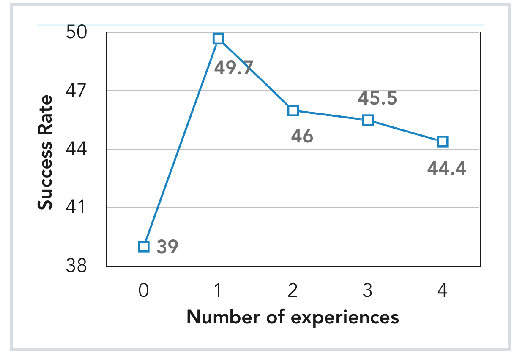
\includegraphics[width=0.61\linewidth]{figures/retrieved_experience_count.pdf}
\caption{检索更多经验并未持续改善成功率。来源：官方课件第41页矢量裁图；相关口述区间01:10:19--01:11:45。设置为 WebArena-Shopping、Gemini-2.5-Flash；图源为官方PDF，非视频截图。}
\label{fig:l4-over-retrieval}
\end{figure}

讲者区分了两种可能原因。第一，记忆库中缺少足够相似的任务，追加的经验本来就不相关。此时，检索数量增加无法创造库里不存在的知识；提高任务覆盖和检索质量才可能改善问题。第二，模型难以正确利用多个经验，可能被无关内容分散注意力。此时，训练模型识别相关性、忽略干扰，可能比继续扩充上下文更有帮助。图表说明了退化现象，但没有单独验证哪种原因占主导。

这个实验也不能推出“永远只检索一条”。一个经验可能覆盖搜索，却无法覆盖验证结果或处理例外；另一个任务可能确实需要多个互补技能。值得保留的是检索预算需要通过任务结果验证，记忆质量、相关性与模型利用能力都影响这个预算。

\subsection{记忆巩固：给函数库安排退出机制}

检索控制作用于当前任务的上下文，记忆巩固作用于长期保存的库。随着任务不断到来，模型可能生成许多只用过一次、功能重复或已失效的函数。如果这些函数长期保留，选择与理解工具的成本也会增长。讲者用缓存作类比：观察一个条目在过去的使用频率，低频条目可以被移除，以减少上下文负担。

TroVE 把这个想法落实为周期性的函数库裁剪。直觉是，随着已处理样本变多，一个函数需要表现出一定的复用频率，才值得继续占据库中的位置。课件给出的阈值已与 TroVE 原论文第3.3节核对，删除条件如下：

$$
u(f)<\lambda(n),\qquad \lambda(n)=\frac{1}{2}\log_{10}(n).
$$
\begin{itemize}
\item $f$：库中的一个已归纳函数。
\item $u(f)$：截至当前检查时，函数 $f$ 已被使用的次数。
\item $n$：到目前为止已经处理的样本数，取正数。
\item $\lambda(n)$：随样本数量缓慢增长的最低使用次数阈值。
\item $\frac{1}{2}$：原论文采用的阈值系数，属于该方法的设计选择。
\item $\log_{10}$：以10为底的对数；这里没有改写为自然对数。
\item $<$：严格低于阈值时移除；计数恰好达到阈值不满足删除条件。
\end{itemize}

例如，处理100个样本时阈值为1；处理10,000个样本时阈值为2。阈值随任务流增长，增长速度很慢。这是一种容易实现的使用频率启发式，衡量的是已发生的复用。它不能单独判断一个低频函数是否对罕见而重要的任务有价值，也不能说明一个高频函数是否始终适用。

\begin{figure}[H]
\centering
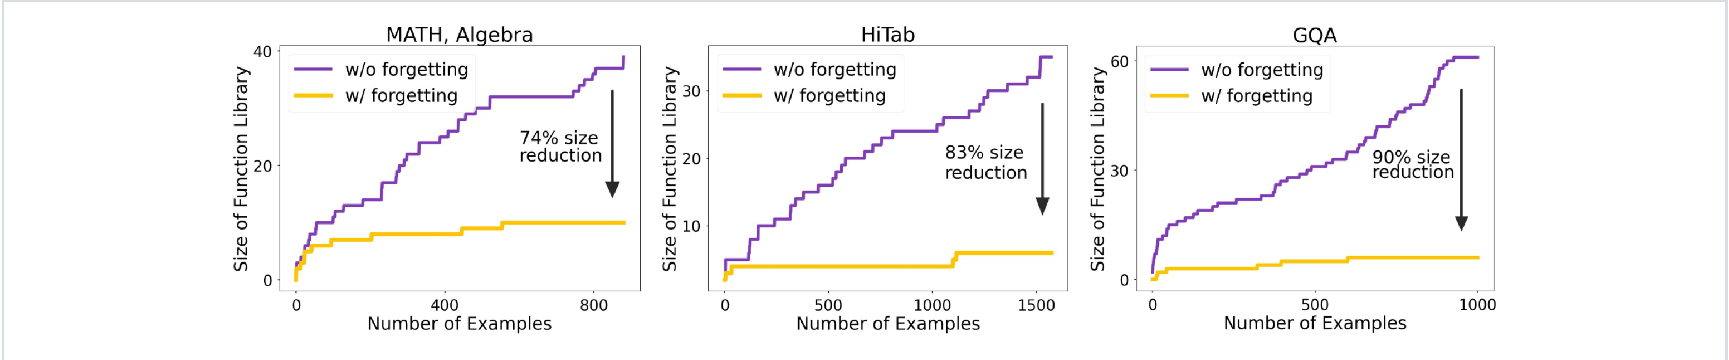
\includegraphics[width=\linewidth]{figures/trove_library_trimming.pdf}
\caption{TroVE 中有无遗忘机制的函数库规模。来源：官方课件第42页矢量裁图；相关口述区间01:11:45--01:12:26。图源为官方PDF，非视频截图。}
\label{fig:l4-trove-trimming}
\end{figure}

图中横轴为已经看到的样本数量，纵轴为函数库大小。紫线表示不使用遗忘，黄线表示使用遗忘；在 MATH 的代数子集、HiTab 和 GQA 三个设置中，图中标示的库规模下降分别为74\%、83\%和90\%。这些曲线直接展示了\textbf{规模控制}，没有在同一图里展示任务成功率。讲者进一步指出，更小的库可以提高效率，并可能在模型被无关工具干扰时改善成功率；后一个效果需要另外的结果支持。

\begin{knowledgebox}{课件补充：技能的收益可能随任务类型改变}
第42页还链接了 \emph{Not All Skills Help: Measuring and Repairing Agent Knowledge}；这一论文名称及具体研究没有在本段口述中展开。论文通过在保留任务上随机屏蔽技能，测量加入技能对结果的影响，发现某些技能帮助一种任务，却妨碍另一种任务。它提示另一条维护路线：除了全局删除，还可以按当前任务屏蔽不适用的技能。该补充强调适用范围，不能用一个平均收益取代任务条件。
\end{knowledgebox}

\subsection{本章小结}

技能库需要同时处理经验的内容、判定的可靠性、检索的选择和长期规模。ReasoningBank 的失败案例说明，失败可以提供查询与浏览策略的教训；三种记忆表示的比较说明，教训怎样表达会影响收益。模拟判定噪声与检索数量消融进一步表明，记忆系统的每一个环节都要接受任务结果检验。TroVE 则给出了一个具体的退出规则，把“持续增加”扩展为“增加与裁剪”。

\subsection{拓展阅读}

\begin{itemize}
\item \href{https://arxiv.org/abs/2509.25140}{ReasoningBank: Scaling Agent Self-Evolving with Reasoning Memory}：第5节和附录C分别对应失败经验、判定校准与检索数量实验；本章图表数值已与论文核对。
\item \href{https://arxiv.org/abs/2401.12869}{TroVE: Inducing Verifiable and Efficient Toolboxes for Solving Programmatic Tasks}：第3.3节给出周期裁剪及阈值。课件补充论文见 \href{https://arxiv.org/abs/2606.15390}{Not All Skills Help: Measuring and Repairing Agent Knowledge}。
\end{itemize}

\clearpage
\section{训练技能归纳：把后续复用放进学习目标}

至此，许多方法仍采用提示模型的方式：让模型观察轨迹，预测哪些内容未来可能有用，再把它们存入记忆。这种做法能利用模型已有的归纳能力，却没有直接训练它为\textbf{未来任务的复用价值}做选择。课件第43页和讲者最后的研究讨论提出了一个自然的下一步：把“保存后是否有用”也纳入训练反馈。

\subsection{为什么当前任务的成功奖励不够}

回到开头的两个购物任务。任务一把 Sony 耳机加入愿望清单，其中包含搜索商品的操作；任务二查询无线键盘的价格范围，也需要搜索。如果任务一完成，奖励只能确认这次加入愿望清单成功。它无法区分两种情况：智能体写了一个未来可以复用的搜索技能，或者它写了一个仅能处理当前商品的临时程序。

要评价保存技能的价值，训练过程需要让任务二真正到来。任务二是否成功、是否用了任务一产生的技能，才能提供与复用有关的反馈。这是跨任务的信用分配问题：较早的存储决定产生效果，要到较晚的执行结果中才能看见。

\begin{figure}[H]
\centering
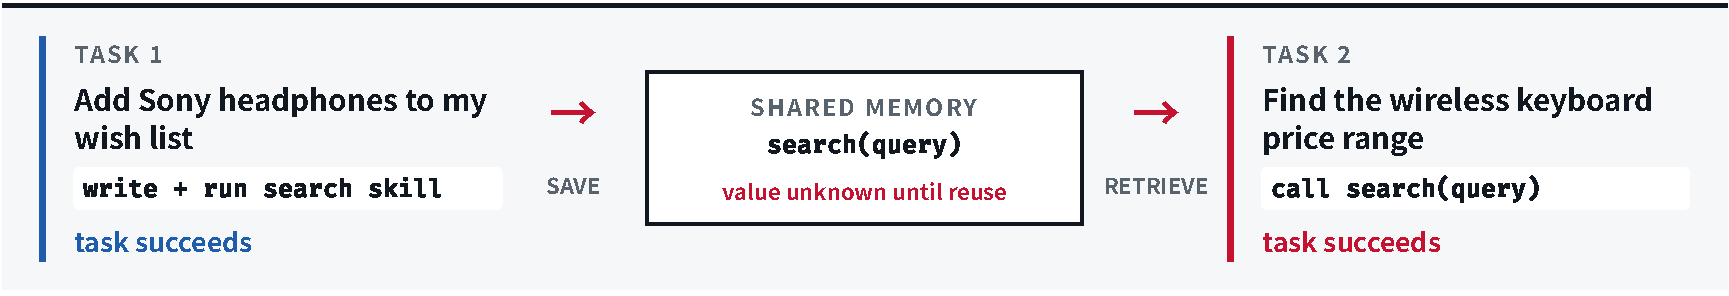
\includegraphics[width=\linewidth]{figures/sage_cross_task_rollout.pdf}
\caption{保存搜索技能的价值需要后续任务揭示。来源：官方课件第43页矢量裁图；相关口述区间01:13:08--01:15:03。图源为官方PDF，非视频截图。}
\label{fig:l4-cross-task-reward}
\end{figure}

\begin{importantbox}{训练样本需要覆盖记忆产生效果的时间跨度}
只观察任务一的结局，无法直接评价为任务二保存技能是否值得。把相关任务依次放入同一次训练展开，让后续任务访问前面产生的记忆，才能给早期归纳和保存行为提供延迟反馈。
\end{importantbox}

\subsection{SAGE 与 AgeMem：两种时间结构}

SAGE 的做法是\textbf{顺序展开相关任务}。它把两个相似任务组成任务链，先执行第一个任务，并把产生的技能保存在共享库中，再执行第二个任务。第二个任务可使用第一个任务留下的技能，因此训练能观察技能的产生与复用。课件采用两个购物任务来说明这一结构；原论文的主要训练设置也使用两个任务，以控制较长任务链的训练成本。

AgeMem 在课件中作为另一条路线出现：把较早的记忆决策和较晚的任务结果放进一条长轨迹。\textbf{论文核对补充：}它联合训练长期记忆与短期上下文管理，轨迹包含信息接触与保存、干扰内容下的上下文管理、以及依赖记忆的最终任务三个阶段；长期记忆跨阶段保留。这使末端结果可以监督前面的存储、检索、更新、压缩与丢弃决定。

两者共享一个训练直觉：把早期记忆行为的后果纳入同一个反馈过程。它们的样本结构与对象不同。SAGE 这里讨论的是两个相关任务间的程序化技能复用；AgeMem 讨论的是一条分阶段长轨迹里的记忆与上下文管理。不能把 AgeMem 写成 SAGE 的两任务购物奖励实验，也不能把 SAGE 的数值归给 AgeMem。

\subsection{奖励成功的复用，而不是仅奖励调用}

后续任务成功，仍不能证明它用到了前面的技能。它可能重新独立解决了任务。因此，SAGE 为成功结果添加了一个与技能复用相关的奖励项。直觉是：任务一要因为“产生了可在任务二成功使用的技能”得到额外反馈，任务二要因为“成功使用了已有技能”得到额外反馈。下面给出原论文第3.2.3节的完整两任务奖励；课件只展示了第一行的简写。

$$
\begin{aligned}
R_1 &= r_1+\mathbf{1}[r_1=1]\cdot\mathbf{1}[r_2=1]\cdot\mathbf{1}_{\mathrm{skill}}(q_2\mid q_1),\\
R_2 &= r_2+\mathbf{1}[r_2=1]\cdot\mathbf{1}_{\mathrm{skill}}(q_2\mid q_1).
\end{aligned}
$$
\begin{itemize}
\item $q_1,q_2$：顺序执行的第一、第二个任务。
\item $r_1,r_2\in[0,1]$：相应任务可验证的结果奖励；取1表示任务完全成功。
\item $R_1,R_2$：加入技能奖励后，用于训练的第一、第二任务奖励。
\item $\mathbf{1}[r_1=1]$、$\mathbf{1}[r_2=1]$：完全成功的指示量，条件成立时为1，否则为0。
\item $\mathbf{1}_{\mathrm{skill}}(q_2\mid q_1)$：任务二是否使用了任务一产生的技能，使用时为1，否则为0；竖线表示技能来源关系。
\item 指示量相乘：所有对应条件同时成立才得到1点额外奖励，任一条件不成立时该项为0。
\end{itemize}

这组奖励有两个值得细读的地方。首先，“调用过技能”并不会单独获得奖金：任务二还必须成功。其次，任务一与任务二的奖金条件并不完全相同。任务一的奖金要求两个任务都成功，并且发生复用；任务二的奖金要求自身成功且发生复用。这样，较早的技能产生与较晚的技能使用都进入学习目标，但各自承担的条件不同。

\begin{warningbox}{复用奖励仍是可观察的代理信号}
记录“任务二用了任务一的技能”，比只观察任务成功更接近复用目标，但它并未单独证明该技能对成功不可或缺。奖励设计需要依赖可检查的行为，任务分布也需要让相关技能确有复用机会。不能把一个技能调用计数直接等同于技能的因果价值。
\end{warningbox}

\subsection{怎样读懂奖励消融的55.4、56.6与60.7}

课件比较了三种训练奖励。仅结果奖励依据各任务的完成情况；任务链奖励在两个训练任务都成功时额外给分，不要求追踪技能使用；技能奖励则包含上面的成功复用条件。这三种设置都使用顺序展开，差别在奖励设计。

\begin{figure}[H]
\centering
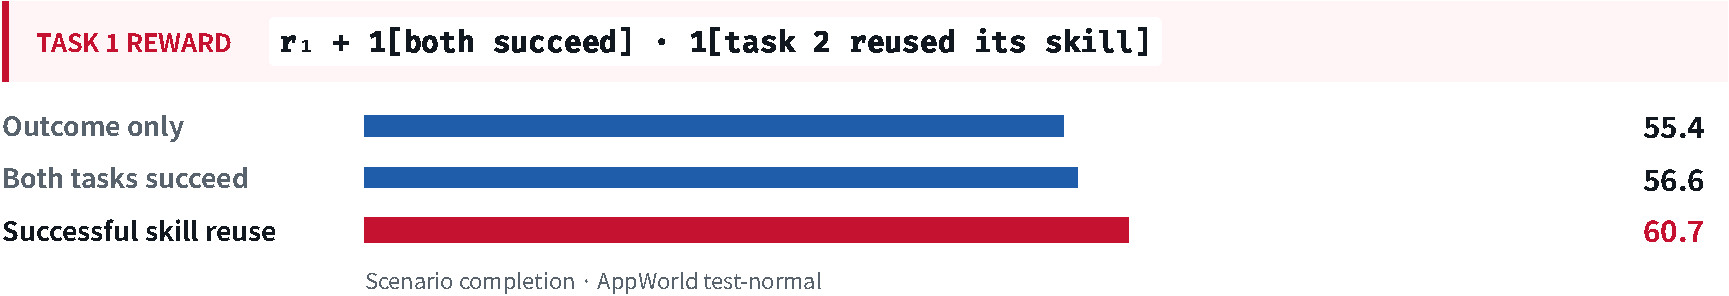
\includegraphics[width=\linewidth]{figures/sage_reward_ablation.pdf}
\caption{SAGE 的奖励消融：仅结果奖励、任务链成功奖励和成功技能复用奖励。来源：官方课件第43页矢量裁图；相关口述区间01:13:53--01:15:03。图源为官方PDF，非视频截图。}
\label{fig:l4-sage-reward-ablation}
\end{figure}

原论文表5确认，图中的55.4、56.6和60.7分别是三种奖励设计在 AppWorld 的 \texttt{test-normal} 上取得的\textbf{场景目标完成率}（Scenario Goal Completion，SGC，\%），基座模型为 Qwen2.5-32B-Instruct。这一评测要求一个场景内的\textbf{三个相似任务全部成功}；训练中的两任务链与评测中的三任务场景是不同的设置。三种奖励对应的单任务目标完成率为69.8\%、67.9\%和72.0\%，因此不能把55.4--60.7称为单任务准确率。

技能奖励比仅结果奖励提高5.3个百分点，比任务链奖励提高4.1个百分点。这个消融支持讲者的结论：在此训练与评测设置中，显式奖励成功的技能复用，比只奖励任务完成或整条任务链完成更有效。它没有证明所有环境都应采用相同的奖金，也没有单独展示开放技能库中的检索难题；论文主要设置在同一场景内保留和复用技能。

\subsection{非可微系统也能接收强化学习反馈}

讲者在01:13:53--01:15:03的实质结尾强调，整个过程可以很复杂：模型产生技能，技能进入外部库，检索过程选择技能，再由另一次执行产生结果。存文件、数据库检索和工具调用通常不是可微运算，但这并不妨碍强化学习优化产生这些决定的模型。训练可以把它们看成执行过程的一部分，根据后续奖励提高有用决定被生成的概率。

这里的“可以优化”有明确的边界：无需对记忆库与环境中的每一步操作求导，不代表无需模型训练，也不保证延迟奖励能轻易解释每个中间决定。关键是在训练展开里保留足够的时间结构，使最终反馈覆盖技能产生、保存和使用。后续课程再介绍具体的强化学习算法，本讲着重说明为什么这种反馈能够指向跨任务记忆。

\subsection{本章小结}

技能归纳的训练目标需要越过当前任务。SAGE 通过两个相关任务的顺序展开，让后续复用产生可观察反馈，再为成功复用添加奖励。AgeMem 则在一条分阶段长轨迹中联合学习记忆和上下文管理。二者都把记忆决策的延迟后果带进训练，但不能混用样本结构、奖励公式或实验结果。课件的 SAGE 消融说明，在特定的 AppWorld 设置中，显式的成功复用奖励提高了场景完成率。

\subsection{拓展阅读}

\begin{itemize}
\item \href{https://aclanthology.org/2026.acl-long.69/}{Reinforcement Learning for Self-Improving Agent with Skill Library}：SAGE 的正式论文。第3.2.3节给出两任务奖励，表5给出课件采用的奖励消融，附录J.1定义对照奖励。
\item \href{https://aclanthology.org/2026.acl-long.981/}{Agentic Memory: Learning Unified Long-Term and Short-Term Memory Management for Large Language Model Agents}：AgeMem 的正式论文，可对照理解分阶段长轨迹与记忆操作作为动作的训练方式。
\end{itemize}

\clearpage
\section{总结与延伸}

\subsection{本讲形成的完整问题链}

本讲从重复任务中的共同结构出发：搜索商品、填写表单或检查代码，不同任务可能反复需要相同的局部行为。如果每次都从零决定这些动作，智能体会重复探索，也可能重复犯错。外部记忆让经验跨任务保存；技能把其中的行动知识组织成未来可以使用的指导或程序。

由此得到一条贯穿全讲的问题链：\textbf{先决定保存什么，再决定怎样表示，随后决定何时使用，最后检查是否仍值得保留。}完整经历保留更多细节，但成本较高；事实保存环境或用户信息；失败教训解释需要避免的条件；文字技能保留解释与适应空间；代码技能把一部分行动交给可执行程序，并带来测试、组合与效率的机会。表示不同，模型在新任务中承担的工作也不同。

本讲介绍的人类编写与经验归纳可以相互衔接。人类知道明确的偏好、规范或检查步骤时，可以先写成技能；智能体有大量交互机会时，可以从经历中提出候选技能；可执行反馈帮助检查候选，人类也可以查看和修改这些外部材料。这里真正需要管理的是长期留下的行为指导：它的适用条件、证据和更新责任应当能够被理解。

\begin{importantbox}{技能库的价值来自未来行动}
一条经验被保存、一个函数被生成、一个技能被调用，都只是中间事件。它们是否值得，最终要看后续任务是否更容易完成、交互是否更有效率，以及保存的行为是否在当前环境中仍然适用。技能归纳、检索、验证和维护因此构成一个循环。
\end{importantbox}

\subsection{讲者结尾保留的研究方向}

实质性的口述结尾继续沿着这个循环讨论训练。强化学习能够为复杂、非可微的记忆使用过程提供反馈；成功复用奖励已经给出了初步证据。讲者接着提出，未来还可以在奖励中加入控制技能库大小的项，使归纳过程受到正则化约束，减少过度拟合和无节制扩张。这是讲者提出的未来方向，课件没有给出该奖励的具体公式或验证结果。

这一设想与前面的 TroVE 相呼应。TroVE 在推理过程中用使用频率规则裁剪函数库；训练中的库大小惩罚则希望模型在生成与保存阶段就考虑成本。二者作用的位置不同，也都需要与任务收益一起衡量：库更小可能更容易选择，但丢掉真正有用的能力也会降低未来表现。

把本讲的证据放在一起，可以看见几个尚未被统一解决的问题：怎样把成功与失败转化为可靠技能，怎样处理判定器的结构性错误，怎样检索多个互补技能而避免干扰，以及怎样让训练获得足够长的反馈跨度。讲者的结尾把这些问题留作技能归纳与管理的研究空间，没有提出一种覆盖所有场景的固定配方。

\subsection{课件讨论补充：应该让什么长期存在}

\textbf{以下讨论来自官方课件第44--45页，视频没有逐项展开。}它们把全讲的取舍整理为四组选择，并提出三个讨论问题：应该保存经历、事实、教训、文字技能还是代码，何时删除或修订技能，以及人类与智能体怎样分配创建和使用技能的工作。

\begin{center}
\small
\begin{tabularx}{\linewidth}{@{}p{0.25\linewidth}X@{}}
\toprule
课件中的取舍 & 阅读本讲时可用的判断依据\\
\midrule
具体经历与一般技能 & 是否需要原始细节作为证据，还是需要把变化的输入抽出来，复用共同的行动结构。\\
灵活指导与固定执行 & 环境是否经常变化；哪些步骤需要模型在现场判断，哪些步骤可以交给经过检验的程序。\\
复用已有内容与探索替换 & 当前技能是否匹配环境；继续调用是否重复失败；是否存在更可靠或更省步骤的实现。\\
扩大记忆与更新、合并、删除 & 新条目是否提供了现有内容没有覆盖的能力；重复、冲突或过时内容是否妨碍选择。\\
\bottomrule
\end{tabularx}
\end{center}

这些问题可以用本讲同一个购物例子来理解。耳机的价格是需要更新的事实；一次具体搜索的页面与结果属于经历；“宽泛查询加反复翻页会耗尽预算”可以成为教训；查询与筛选原则可以写成文字技能；可靠的搜索实现则可以成为代码技能。它们保存的是不同种类的信息，更新频率与验证方式也应随之变化。

\subsection{课件讨论补充：谁负责记忆决策}

第45页进一步按生命周期分配人类与智能体的工作。这里的表格是对课件的中文整理，不是讲者在视频中逐项作出的口头结论。

\begin{center}
\small
\begin{tabularx}{\linewidth}{@{}p{0.19\linewidth}XX@{}}
\toprule
决策 & 人类投入更有价值的条件 & 智能体投入更有价值的条件\\
\midrule
编写或归纳 & 技能或政策已经明确。 & 需要通过交互才能发现有效做法。\\
验证并准入 & 正确性取决于规范，或错误后果重大。 & 结果可执行，验证成本较低。\\
选择并使用 & 罕见例外需要结合情境判断。 & 技能选择反复出现，并能产生反馈。\\
持续维护 & 责任追踪需要明确的所有者。 & 环境变化能从结果中看见，并可修复。\\
\bottomrule
\end{tabularx}
\end{center}

这个分工与外部技能的可检查性相连：材料可以由智能体提出，也可以被人阅读、修改和重新验证。即使创建过程自动化，保存下来的规则仍然需要有适用范围；即使维护由智能体执行，变化也需要能从任务结果中被观察。把这些条件写清楚，才能让跨任务经验成为可以持续管理的知识。

\subsection{本章小结}

本讲把“记住过去”推进为“改进未来行动”。外部记忆提供跨任务保存，技能表示决定如何复用，执行反馈帮助验证，检索与维护决定哪些内容真正进入下一次任务。结尾的训练方向进一步把后续成功与复用回传给早期决策。课件补充的人类与智能体分工，则提醒读者把技能的创建、准入、使用和维护分别放到有证据、有能力承担的位置。

\subsection{拓展阅读}

\begin{itemize}
\item 对照 \href{https://arxiv.org/abs/2401.12869}{TroVE} 与 \href{https://aclanthology.org/2026.acl-long.69/}{SAGE}：前者通过推理过程中的裁剪控制库大小，后者通过跨任务奖励训练技能归纳与使用；这有助于定位讲者提出的“训练时约束技能库规模”处于哪一步。
\item \href{https://arxiv.org/abs/2606.15390}{Not All Skills Help}：作为课件延伸，继续追问同一技能为什么对不同任务产生不同效果，以及按任务选择技能与全局删除技能有什么区别。
\end{itemize}

\end{document}
